

\documentclass[conference]{IEEEtran}



\usepackage[normalem]{ulem}
\usepackage{todonotes}

\newcommand{\mynote}[2]{\todo[inline]{#1 : #2}}
\newcommand{\quotes}[1]{``#1''}
\newcommand{\figref}[1]{Fig.~\ref{fig:#1}}
% correct bad hyphenation here
\hyphenation{op-tical net-works semi-conduc-tor}

\usepackage[per-mode=symbol]{siunitx} 
\usepackage{truonglatexdefs}
\usepackage{subfigure}


\begin{document}
%
% paper title
% Titles are generally capitalized except for words such as a, an, and, as,
% at, but, by, for, in, nor, of, on, or, the, to and up, which are usually
% not capitalized unless they are the first or last word of the title.
% Linebreaks \\ can be used within to get better formatting as desired.
% Do not put math or special symbols in the title.
\title{Five Challenge Problems in Cyber-Physical Systems}


% author names and affiliations
% use a multiple column layout for up to three different
% affiliations
\author{\IEEEauthorblockN{Rahul Mangharam, Houssam Abbas, Madhur Behl, Kuk Jang, Zhihao Jiang, Matthew O'Kelly and Yash Vardhan Pant}
\IEEEauthorblockA{
%Department of Electrical \& Systems Engineering and Department of Computer and Information Science\\
School of Engineering and Applied Sciences\\
University of Pennsylvania\\
Philadelphia, Pennsylvania. USA 19104\\
Email: \{rahulm, habbas, mbehl, jangkj, zhihaoj, mokelly, yashpant\}@seas.penn.edu}}




% use for special paper notices
%\IEEEspecialpapernotice{(Invited Paper)}




% make the title area
\maketitle

% As a general rule, do not put math, special symbols or citations
% in the abstract
\begin{abstract}
The tight coupling of computation, communication and control with physical systems such as actuation of closed-loop medical devices within the human body, peak power minimization by coordination of controllers across large industrial plants, and fast life-critical decision making by autonomous vehicles, present a set of fundamental and unique challenges. Each of these require new approaches at the intersection of multiple scientific, human and systems disciplines. We discuss five such challenges which require creative insights and application of model-based design, control systems, scheduling theory, formal methods, statistical machine learning and domain-specific experimentation. We ask the following questions: 
(1) An autonomous medical device is implanted to control your heart over a period of 5-7 years. How do you guarantee the software in the device provides safe and effective treatment under all physiological conditions?
(2) Electricity prices in the US have summer peaks that are over 32x their average prices and winter peaks that are 86x. How can buildings respond to massive swings in energy prices at fast time scales?
(3) While wireless has been successfully used for open-loop monitoring and tracking, how can we operate closed-loop control systems over a network of wireless controllers. Furthermore, how can we ensure robust, optimal and secure control in the presence of node/link failures and topology changes?
(4) While autonomous vehicles have driven over a million miles, the most basic maneuvers, such as a lane change, are yet to be certified to be safe. How do we verify the safety of the decision controller in an autonomous system under all driving scenarios - in other words how can we provide a driver's license to a self-driving vehicle?
(5) In autonomous vehicles, when the computational resources of the hardware platform become overloaded, the estimation delay can compromise control performance and even stability. How can we co-design adaptive perception algorithms to operate with a fraction of the computing resources while ensuring the control stability and performance?

\end{abstract}

% no keywords




% For peer review papers, you can put extra information on the cover
% page as needed:
% \ifCLASSOPTIONpeerreview
% \begin{center} \bfseries EDICS Category: 3-BBND \end{center}
% \fi
%
% For peerreview papers, this IEEEtran command inserts a page break and
% creates the second title. It will be ignored for other modes.
\IEEEpeerreviewmaketitle


\section{Introduction}
% no \IEEEPARstart
We describe five challenge problems at the foundations of Cyber-Physical Systems (CPS). CPS are the new generation of time-critical and safety-critical Real-Time Embedded Systems where computation and communication are tightly coupled to control large, complex and ``messy" plants. Unlike classical Real-Time Systems where the system is designed in a constrained manner to limit the complexity for predictability, in current CPS, the plants are difficult to model precisely because they are non-deterministic, interactive and often scale to thousands of controllers. We outline research approaches to address these structural concerns in the design of future Cyber-Physical Systems through closed loop modeling, architectures, algorithms and platforms. The eventual goal of efforts such as this is to develop CPS to transform how we interact with and manipulate the physical world, just as the Internet transformed how we interact with information systems.

A key aspect of this cross-cutting work is that each challenge bridges two or more well-established scientific fields such as scheduling theory, control systems, formal methods, statistical machine learning, and experimentation. We illustrate this through five domain-specific problems spanning the safety of closed-loop medical devices, control over wireless, data-driven control of energy systems in volatile price markets, safe decision making in autonomous systems and co-design of computation and control for future automotive systems. We address the foundations of CPS across four themes: Modeling, Architectures, Algorithms and Platforms.
\begin{itemize}
\item \textbf{CPS Modeling:} From verified models into verified code for life-critical systems. We focus on the formal modeling, synthesis and certification of high-confidence medical device software and systems. We describe efforts on both implantable medical devices and physiological control systems to ensure that both the functional and formal aspects are verified, validated and tested within the closed-loop context of their physiological systems. 
\item \textbf{CPS Architectures:} Distributed Control over Wireless Networks. We describe radical architectural approaches for completely in-network computation for robust, optimal and secure control over unreliable infrastructure.
\item \textbf{CPS Algorithms:} Data-driven Controller Synthesis. In highly volatile electricity pricing markets, we required buildings and built environments to rapidly respond to peak pricing spikes. We describe a new data-driven approach for synthesis of control strategies to achieve real-time demand response while ensuring custom climate conditions are maintained.
\item \textbf{CPS Platforms and Test-beds:} To certify autonomous vehicles are safe we describe the experimental challenges with verifying decision controllers and executing them across a range of driving scenarios. As the perception and computation workload increase in such systems, we describe new approaches for the co-design of anytime computation with robust control. This allows the system to trade-off accuracy for faster responses and lower power requirements while ensuring the stability and tracking performance of the vehicle controls. 
\end{itemize}
 \section{The Design of Safe and Effective Closed-loop Medical Devices}
The design of safe, bug-free, and efficient medical device software is challenging, especially in implantable devices that directly control and actuate partially understood organs. However, such design is also essential; safety recalls of pacemakers and implantable cardioverter defibrillators between 1990 and 2000 affected over 600,000 devices~\cite{recalls}. Importantly, 41\% of these recalls were due to software issues~\cite{medstats1}. 
According to the US Food and Drug Administration (FDA), in 1996, 10\% of \emph{all} medical device recalls were caused by software-related issues. This percentage rose to an average of 15\% of recalls from 2008 to 2012. 
 And, surprisingly given these numbers, there is currently no formal methodology or open experimental platform to test the correct operation of medical device software within the \emph{closed-loop} context of the patient~\cite{killedbycode}. Unlike other industries such as aviation and automotive where the safety concern is focused on a well-defined physical plant~\cite{autosar,AVSI}, in the medical device domain patient response is complex and nondeterministic. As a result there are no well-established standards for the development of medical device software that directly control and actuate the patient. For device manufacturers, this has prompted recent interest in applying formal modeling~\cite{hcmdss, challenge2, challenge3} and verification techniques in medical devices software development~\cite{med-form2,med-form1}.\vspace{4pt}
 
\emph{How do you guarantee the device software will not adversely affect the patient under all physiological conditions?}

%problems with testing and need for FM approach
~An effective software verification methodology is therefore needed for the risk analysis and certification of medical device software during the FDA's pre-market submission phase. Testing medical device software currently is ad hoc, open loop, and very expensive~\cite{testing_imd, Vip}. Test generation must be interactive and adaptive and must consider the current state of the patient when generating the next input in a way that advances the purpose of the test. The problem, therefore, becomes one of controller synthesis and cannot be addressed by an off-the-shelf model checker~\cite{rushby}. The key challenge is in the generation of \emph{physiologically relevant} software that does not provide inappropriate therapy or adversely affect the patient. This requires validated patient models of the appropriate abstraction levels and that testing is conducted within the closed-loop context of the patient model.

%building blocks - closed-loop, modeling->synthesis, integrated models, translation
Consequently, there is a need for fundamentally novel approaches to the closed-loop modeling, analysis, and design of medical cyber-physical systems, as well as the development of holistic, heterogeneous physiological models, approaches, and tools that address the many different physical, functional and logical aspects of the device and patient interaction. The scientific agenda of this research on medical cyber-physical systems is to unify theories of formal methods, control of physiological systems, communication and computing systems. Our early efforts are conducted with implantable medical devices, such as cardiac pacemakers and defibrillators, and physiological control systems such as infusion pumps with networks of discrete sub-systems. Both feature tight coupling with the patient-in-the-loop, exposing safety and efficacy risks of autonomous and automatic control of the body.\vspace{4pt}

%focus 1
\textbf{1. Implantable Medical Devices - Cardiac Pacemakers:}
~The human heart is perhaps the most important real-time system, generating electrical impulses that determine the heart's rhythm and proper function. Irregularities with timing, i.e. cardiac arrhythmias, cause inefficient and unsafe function of the blood-oxygen system, necessitating the maintenance of the heart rate artificially. The cardiac pacemaker is a rhythm management device that maintains the minimum heart rate and  synchrony between its chambers, thereby improving the condition of patients with cardiac arrhythmias. Cardiac rhythm management devices have grown in complexity with over 80,000 to 100,000 lines of code~\cite{pauljones}. The primary approach to system-level testing of medical devices is unit testing using a playback of pre-recorded electrogram and electrocardiogram signals. This tests if the input signal triggers a particular response by the pacemaker but cannot evaluate if the response was appropriate for the patient condition. Furthermore, this approach of {\em open loop} ``tape testing'' is unable to check for safety violations due to inappropriate stimulus by the pacemaker. Pacemaker Mediated Tachycardia (PMT), a condition where the pacemaker inappropriately drives the intrinsic heart-rate toward the maximum rate, is a strong example of why we need an interactive and adaptive {\em closed-loop} verification and testing of such systems. With a tape test, PMT would not be observed and the response of the pacemaker could be classified as appropriate therapy.
%%%%%%%%%%%%%%%%%%%%%%%%%%%%%%%%%%%%%%%%%%%%%%%%%%%%%%
\begin{figure}[t]
	\centering
	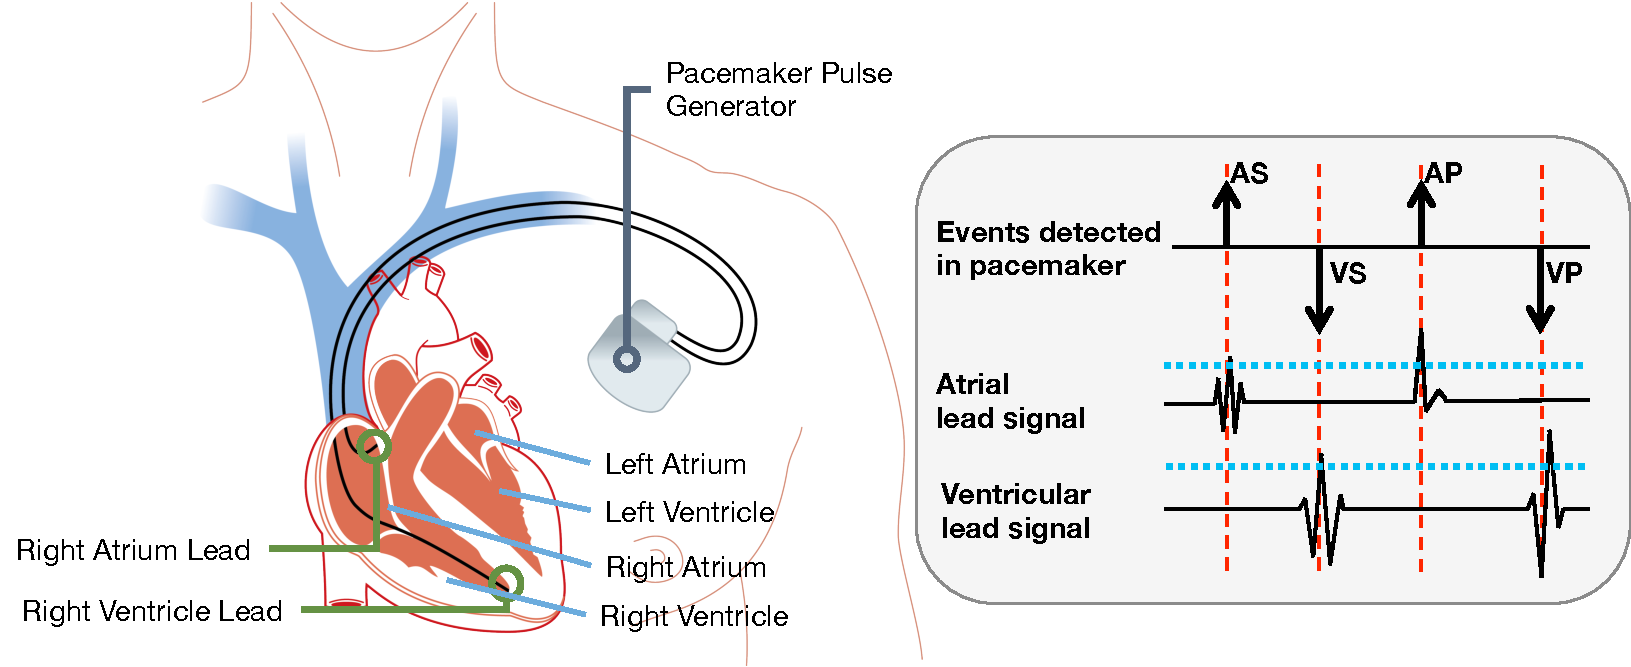
\includegraphics[scale=0.33]{figs/fig1pacemaker.pdf}
	\caption{\small Pacemaker operating in a closed-loop with the heart. The leads sense cardiac electrophysiological activity from inside the heart tissue (AS/VS = Atrial/Ventricular Sense event) and actuate the heart (AP/VP = Atrial/Ventricular Pacing event to maintain the heart rate.}
	\vspace{-20pt}
	\label{fig:pacemaker}
\end{figure}
%%%%%%%%%%%%%%%%%%%%%%%%%%%%%%%%%%%%%%%%%%%%%%%%%%%%%%
\begin{figure}[!b]
	\centering
	\vspace{-20pt}
	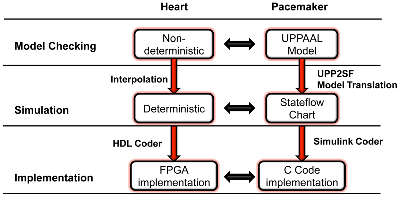
\includegraphics[scale=1.2]{figs/model_based_b.pdf}
	\caption{\small From closed-loop verification to simulation-based testing, code generation and platform evaluation}
	\label{fig:med_overview}
\end{figure}
%%%%%%%%%%%%%%%%%%%%%%%%%%%%%%%%%%%%%%%%%%%%%%%%%%%%%%
%%%%%%%%%%%%%%%%%%%%%%%%%%%%%%%%%%%%%%%%%%%%%%%%%%%%%%
\begin{figure*}
	\centering
	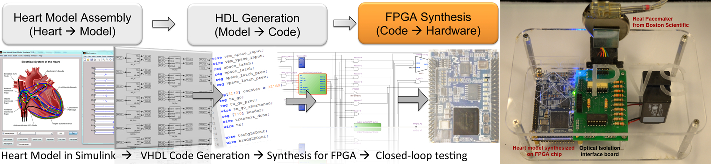
\includegraphics[scale=1.4]{figs/pvs_toolchain.pdf}
	\caption{\small From verified models to verified code: Translating models to a heart-on-a-chip platform for closed-loop testing of cardiac devices}
	\vspace{-10pt}
	\label{fig:pvs_toolchain}
\end{figure*}
%%%%%%%%%%%%%%%%%%%%%%%%%%%%%%%%%%%%%%%%%%%%%%%%%%%%%%

Our proposed model-based design (MBD) for Medical CPS begins with developing integrated functional and formal heart models that interact with real and modeled pacemakers for closed-loop verification and testing~\cite{vhm_proc}. As shown from the top of \figref{med_overview}, the heart-pacemaker closed-loop systems is first modeled abstractly to facilitate verification of the basic pacemaker design with maximum coverage~\cite{vhm_tacas12}. In our case, we use timed automata~\cite{timed_automata, timed-aut} and the UPPAAL model checker~\cite{BDL04, uppaal, uppaal_tut} at this design stage. Next, the models are translated to more detailed models that take into account the complex dynamics of the heart and interaction with more detailed pacemaker model~\cite{vhm_ecrts10, vhm_embc11,vhm_iccps11}. We use Stateflow and Simulink~\cite{stateflow, volkswagen} at this design stage. These models are validated by physicians for their clinical relevance. The automatic model translation procedure, from UPPAAL to Stateflow, ensures that abstract models used for verification over-approximate the more detailed models used downstream~\cite{vhm_rtas12}. Once the detailed models pass simulation-based testing with closed-loop dynamics, they are automatically generated into code and are subject to platform-level integration testing~\cite{vhm_website} as shown in \figref{pvs_toolchain}. This MBD approach ensures the closed-loop safety properties are retained through the design toolchain and facilitates the development of verified software from verified models.\vspace{4pt}

%focus 2
\textbf{2. Physiological Control Systems:}
~The understanding of closed-loop safety analysis of single-system devices such pacemakers has naturally broadened our work to physiological control systems featuring multiple networked devices with the patient-in-the loop~\cite{pcs_iccps10}. Such a clinical scenario is viewed as a control system, in which the patient is the plant, bedside monitors are sensors and drug infusion pumps are actuators~\cite{hcmdss}.  In this setup, caregivers traditionally perform the role of the controller. In many cases automatic controllers for drug infusion can reduce the burden on the caregiver and avoid human errors. However, vendors of medical equipment continue to avoid closed-loop scenarios due to an insufficient understanding of the human body's response to treatment. Furthermore, a particular challenge arises from the complex interplay between the continuous dynamics of the patient's reaction to treatment, and discrete controller and network. 
%Despite many medical devices being able to send sensed data across the network, only few modern medical devices can be controlled remotely. 
%%%%%%%%%%%%%%%%%%%%%%%%%%%%%%%%%%%%%%%%%%%%%%%%%%%%%%
\begin{figure}[!b]
	\centering
	\vspace{-10pt}
	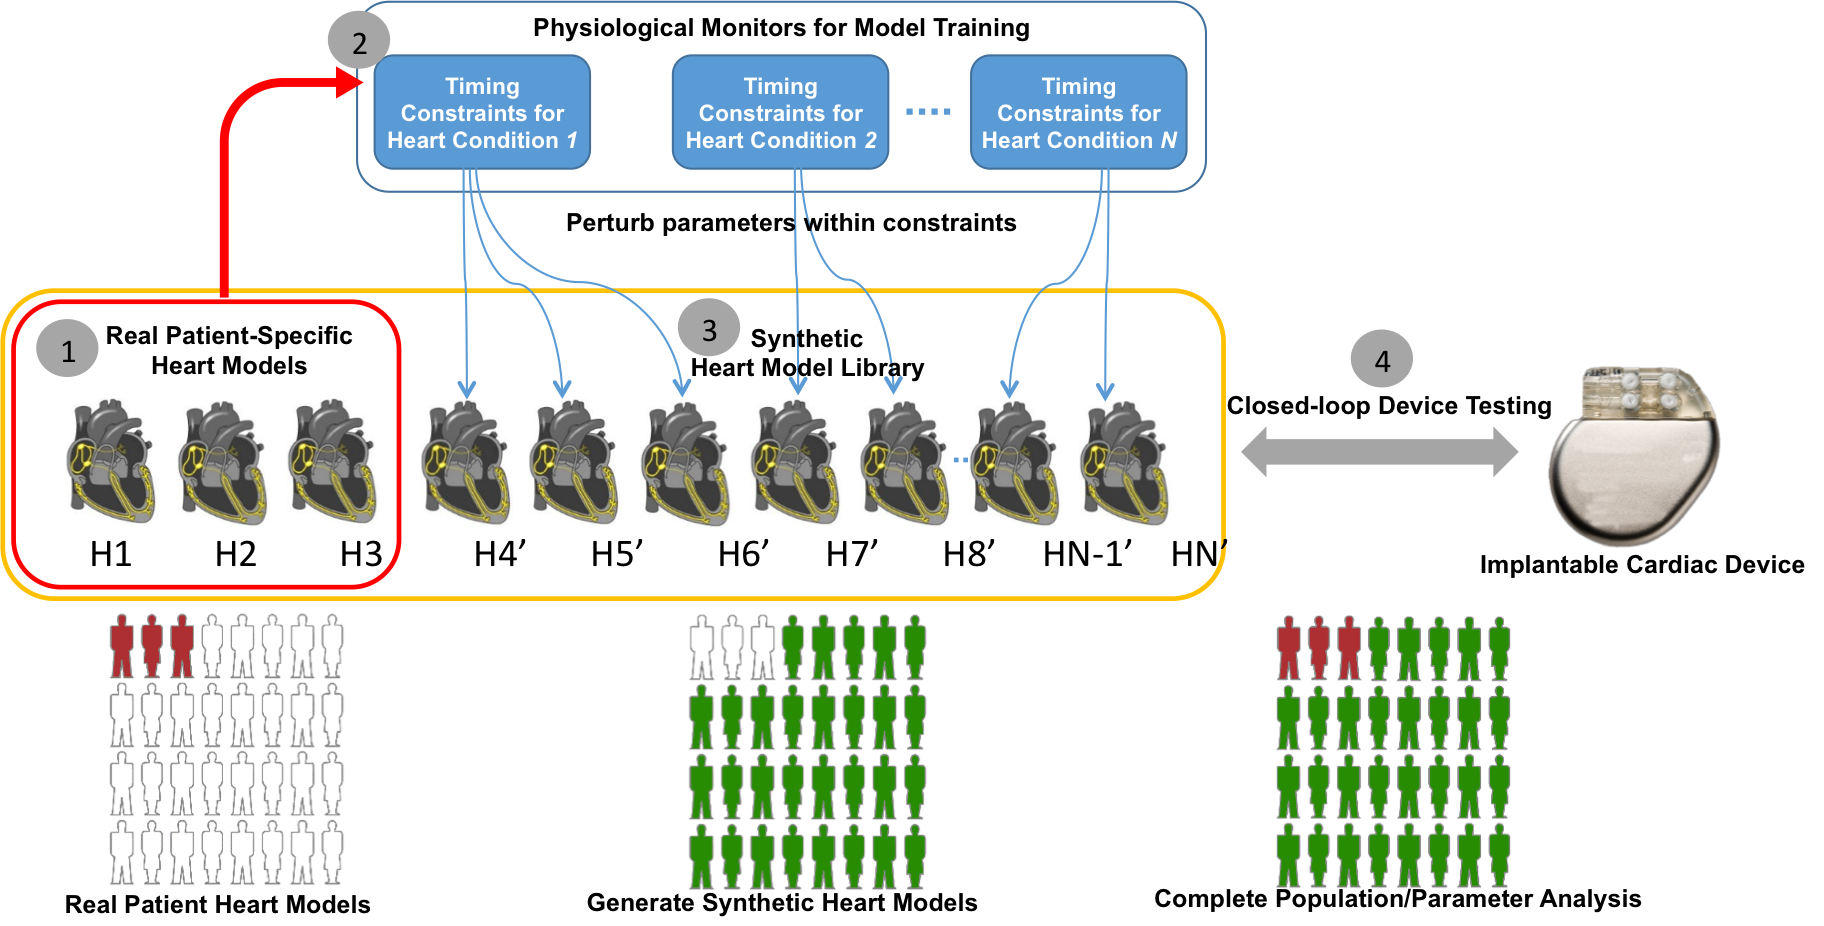
\includegraphics[scale=0.3]{figs/mbct.png}
	\caption{\small Model-based Clinical Trials}
	\label{fig:mbct}
\end{figure}
%%%%%%%%%%%%%%%%%%%%%%%%%%%%%%%%%%%%%%%%%%%%%%%%%%%%%%
Consequently, there is a need for model driven safety analysis of closed-loop medical systems within uncertain parameters. Both the abstract, formal model and the detailed, informal model are needed in the process of verification, validation, and regulatory approval of closed-loop medical device systems.  Formal models allow us to exhaustively explore the possible behaviors of the system and prove its safety, detailed models allow us to use high-fidelity simulation that take real system dynamics into account.  Both kinds of results can be used to make the case for regulatory approval if the abstract model is guaranteed to over-approximate the patient's dynamics with respect to the control algorithms used.\vspace{4pt}

\textbf{3. Model-based Clinical Trials:}
~Regulatory authorities require that the safety and efficacy of a new high-risk medical device be proven in a Clinical Trial (CT), in which the effects of the device on a group of patients are compared to the effects of the current standard of care. 
Phase III trials can run for several years, cost millions of dollars, and pose an inherent risk to the patients by exposing them to an unproven device.
With the use of computational modeling and simulation, we would like to investigate how to use a large model-based synthetic group of patients and device models to improve the planning and execution of a CT so as to increase the chances of a successful trial.

As an example, we apply our initial efforts are in applying it to a real CT that compares two algorithms within implantable cardioverter defibrillators (ICDs) for the detection of potentially fatal cardiac arrhythmias~\cite{RIGHT}. 
In 2011, a CT posited that one algorithm (Boston Scientific's) would be better than the other (Medtronic's) but the results of the trial were opposite to this hypothesis~\cite{RIGHTresults}. 
We begin by modeling the heart and processing 100's of real patients' electrogram signals, mapping the timing and morphology components of the signals to the heart model. 
This is followed by generating a population of 10,000+ synthetic heart models, by perturbing the parameters of the initial heart models for different arrhythmias, and implementing diagnostic algorithms of two very commonly used ICD platforms in the USA, i.e. Boston Scientific and Medtronic.
We conducted conformance testing to validate our device models against real ICDs. 
Now, using the closed-loop of the device models and synthetic patient population we conducted multiple trials to compare the performance of the two algorithms to appropriately discriminate between potentially fatal ventricular tachycardias (VT) and non-fatal SupraVentricular Tachycardias (SVTs). 

The results of our model-based clinical trials (MBCT) indicate we could have accurately predicted this with our model, i.e. that Boston Scientific's algorithm was less able to discriminate between SVT and VT and so may lead to inappropriate therapy.
We further demonstrated that the result continues to hold if we vary the characteristics of the synthetic population and device parameters.
% - thus indicating that the CT was unlikely to prove the desired effect. 
While MBCTs do not seek to replace a CT, they may provide early insight into the factors which affect the outcome at a fraction of the cost and duration and without the ethical issues.
This effort is an early step towards using computer modeling as regulatory-grade evidence for medical device certification. 

 
\section{Data-Driven Modeling, Control and Tools for Cyber-Physical Energy Systems}

In 2013, a report by the U.S. National Climate Assessment provided evidence that the most recent decade was the nation's warmest on record~\cite{melillo2014climate} and 2015 is very likely to become the hottest year on record since the beginning of weather recording in 1880~\cite{noaa}. 
Heat waves in summer and polar vortexes in winter are growing longer and pose increasing challenges to an already over-stressed electric grid. 

Furthermore, with the increasing penetration of renewable generation, the electricity grid is also experiencing a shift from predictable and dispatchable electricity generation to variable and non-dispatchable generation. 
This adds another level of uncertainty and volatility to the electricity grid as the relative proportion of variable generation vs. traditional dispatchable generation increases.
%The organized electricity markets across the world all use some variant of real-time price for wholesale electricity. 
%The real-time electricity market at PJM, one of the world's largest independent system operator (ISO), is a spot market where electricity prices are calculated at five-minute intervals based on the grid operating conditions. 
The volatility due to the mismatch between electricity generation and supply further leads to volatility in the wholesale price of electricity.
For \eg the polar vortex triggered extreme weather events in the U.S. in January 2014, which caused many electricity customers to experience increased costs.
Parts of the Pennsylvania-New Jersey-Maryland (PJM) electricity grid experienced a $86$ fold increase in the price of electricity from $\$31/\si{\mega\watt\hour}$ to $\$2,680/\si{\mega\watt\hour}$ in a matter of a few minutes~\cite{volatility}. 
Similarly, the summer price spiked $32$ fold from an average of $\$25/\si{\mega\watt\hour}$ to $\$800/\si{\mega\watt\hour}$ in July of 2015.
%Such events show how unforeseen and uncontrollable circumstances can greatly affect electricity prices that impact ISOs, suppliers, and customers. 
Energy industry experts are now considering the concept that extreme weather, more renewables and resulting electricity price volatility, could become the new norm.

\begin{figure}[t]
\centering
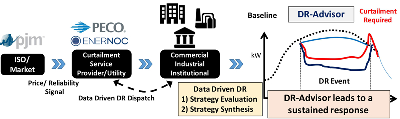
\includegraphics[width=0.9\columnwidth]{figs/demandresponse}
\caption{Majority of DR today is manual and rule-based. The fixed rule based DR is inconsistent and could under-perform compared to the required curtailment, resulting in DR penalties. Using data-driven models DR-Advisor uses DR strategy evaluation and DR strategy synthesis for a sustained and sufficient curtailment.}
\label{fig:demand_response}
\vspace{-10pt}
\end{figure}

Across the United States, electric utilities and independent service operators (ISOs or grid coordinators) are devoting increasing attention and resources to demand response (DR)~\cite{goldman2010coordination}. It is considered as a reliable means of mitigating the uncertainty and volatility of renewable generation and extreme weather conditions and improving the grid's efficiency and reliability.
The potential demand response resource contribution from all U.S. demand response programs is estimated to be nearly 72,000 megawatts (MW), or about 9.2 percent of U.S. peak demand~\cite{federal2008assessment} making DR the largest virtual generator in the U.S. national grid.
The annual revenue to end-users from DR markets with PJM ISO alone is more than $\$700$ million~\cite{pjm}. 
Global DR revenue is expected to reach nearly $\$40$ billion from 2014 through 2023~\cite{navigant}.


%The volatility in real-time electricity prices poses the biggest operational and financial risk for large scale end-users of electricity such as large commercial buildings, industries and institutions~\cite{Mulhall2014327}; often referred to as \textit{C/I/I} consumers. 
In order to shield themselves from the volatility and risk of high prices, such consumers must be more flexible in their electricity demand. 
Consequently, large commercial, industrial and institutional customers are increasingly looking to demand response programs to help manage their electricity costs.
As shown in \figref{demand_response}, DR programs involve a voluntary response of a building to a price signal or a load curtailment request from the utility or the curtailment service provider. 
Upon successfully meeting the required curtailment level the end-users are financially rewarded, but may also incur penalties for under-performing and not meeting a required level of load curtailment.


\subsection{Challenges}

On the surface demand response may seem simple. Reduce your power when asked to and get paid. 
However, in practice, one of the biggest challenges with end-user demand response for large scale consumers of electricity is the following: \emph{Upon receiving the notification for a DR event, what actions must the end-user take in order to achieve an adequate and a sustained DR curtailment?} 
This is a hard question to answer because of the following reasons:\vspace{4pt}

\textbf{1. Modeling complexity and heterogeneity:}
~Unlike the automobile or the aircraft industry, each building is designed and used in a different way and therefore, it must be uniquely modeled. 
%Learning predictive models of building's dynamics using first principles based approaches (\eg with EnergyPlus~\cite{Crawley2001319}) is very cost and time prohibitive and requires retrofitting the building with several sensors~\cite{sturzeneggermodel};
The user expertise, time, and associated sensor costs required to develop a model of a single building (\eg with EnergyPlus~\cite{Crawley2001319}) is very high~\cite{sturzeneggermodel} - often taking 5-12 months to model and tune the model.
This is because usually a building modeling domain expert requires the geometry of a building from the building design and equipment layout plans, detailed information about material properties, and of  equipment and operational schedules. \vspace{4pt}
%There is always a gap between the modeled and the real building and the domain expert must then manually tune the model to match the measured data from the building~\cite{new2012autotune}. 
%\item \textbf{Limitations of rule-based DR}: The building's operating conditions, internal thermal disturbances and environmental conditions must all be taken into account to make appropriate DR control decisions, which is not possible with using rule-based and pre-determined DR strategies since they do not account for the state of the building but are instead based on best practices and rules of thumb. The performance of a rule-based DR strategy is inconsistent and can lead to reduced amount of curtailment which could result in penalties to the end-user. In our work, we show how a data-driven DR algorithm outperforms a rule-based strategy by $17\%$ while accounting for thermal comfort.
%Rule based DR strategies have the advantage of being simple but they do not account for the state of the building and weather conditions during a DR event.
%Despite this lack of predictability, rule-based DR strategies account for the majority of DR approaches.

\textbf{2. Control complexity and scalability:}
~Upon receiving a notification for a DR event, the building's facilities manager must determine an appropriate DR strategy to achieve the required load curtailment. 
These control strategies can include adjusting zone temperature set-points, supply air temperature and chilled water temperature set-point, dimming or turning off lights, decreasing duct static pressure set-points and restricting the supply fan operation \etc 
For a large building, it is difficult to asses the effect of one control action on other sub-systems and on the building's overall power consumption because the building sub-systems are tightly coupled. 
%Consider the case of the University of Pennsylvania's campus, which has over a hundred different buildings and centralized chiller plants. In order to perform campus wide DR, the facilities manager must account for several hundred thousand set-points and their impact on the different buildings. 
Therefore, it is extremely difficult for a human operator to accurately gauge the building's or a campus's response.\vspace{4pt}

\textbf{3. Interpretability of modeling and control:}
~Predictive models for buildings, regardless how sophisticated, lose their effectiveness unless they can be interpreted by human experts and facilities managers in the field.
For \eg artificial neural networks (ANN) obscure physical control knobs and interactions and hence, are difficult to interpret by building facilities managers.
Therefore, the required solution must be transparent, human centric and highly interpretable.

%The goal with data-driven methods for cyber-physical energy systems is to make the best of both worlds; i.e. simplicity of rule based approaches and the predictive capability of model based strategies, but without the expense of first principle or grey-box model development.

\subsection{Real-Time Data-driven Demand Response}

We have developed a method called DR-Advisor (Demand Response-Advisor)~\cite{dr_advisor}, which acts as a recommender system for the building's facilities manager and provides the power consumption prediction and control actions for meeting the required load curtailment and maximizing the economic reward.  
Using historical meter and weather data along with set-point and schedule information, DR-Advisor builds a family of interpretable regression trees to learn non-parametric data-driven models for predicting the power consumption of the building (Figure~\ref{fig:overview}).
DR-Advisor can be used for real-time demand response baseline prediction, strategy evaluation and, most importantly, for control synthesis, without having to learn first principles based models of the building:\vspace{4pt}

\textbf{1. DR Baseline Prediction:} A baseline is an estimate of the electricity that would have been consumed by a customer in the absence of a demand response event. Typical demand response programs rely upon financial incentive for customers based on the extent to which they reduce their energy consumption and therefore require a reliable system to measure the energy reduction. For this reason the measurement and verification of demand response is the most critical component of any DR program. Using regression trees based approaches, DR-Advisor achieves a prediction accuracy of $93\%$ to $98.9\%$ for baseline estimates of eight buildings on the Penn campus by just analyzing data as shown in Figure~\ref{fig:overview}.\vspace{4pt}
\begin{figure}[t]
\centering
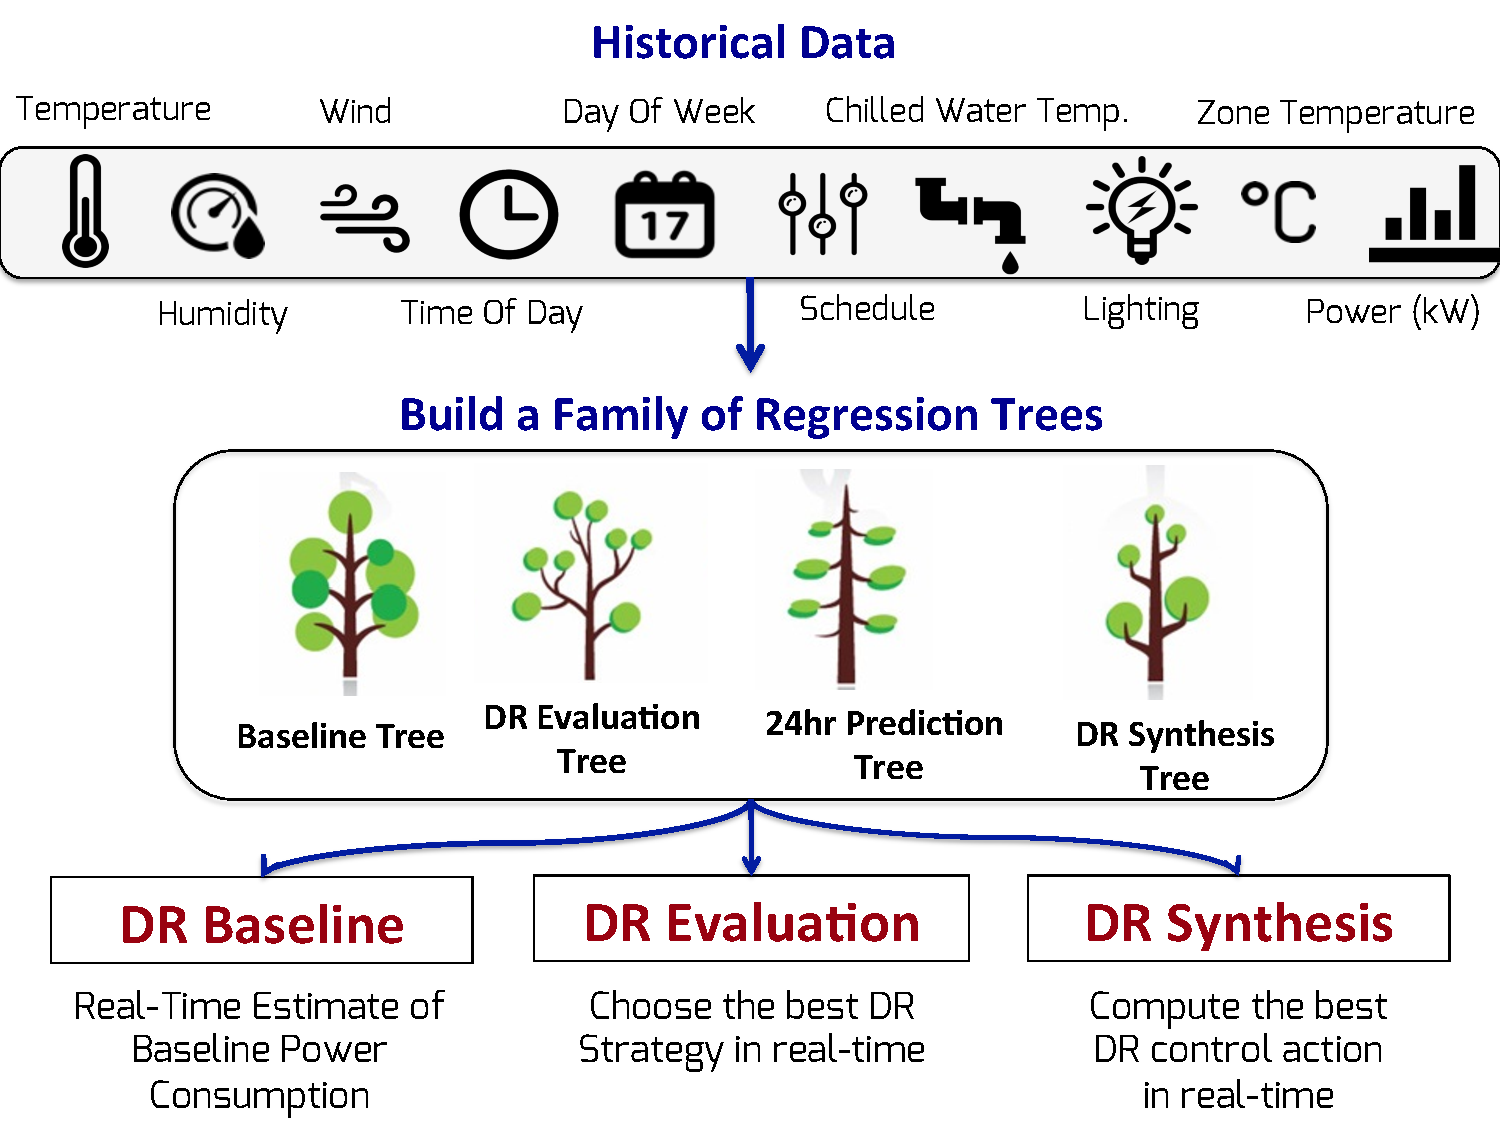
\includegraphics[width=0.85\columnwidth]{figs/overview.pdf}
\vspace{-3pt}
\caption{DR-Advisor Architecture for real-time demand response}
\label{fig:overview}
\vspace{-16pt}
\end{figure}

\textbf{2. DR Strategy Evaluation:} A DR strategy refers to what sequence of control actions, and at what times, a system (lighting, HVAC or plug loads) will actuate. 
Furthermore, there could be several of such fixed DR strategies, but only one specific strategy can be used at a time. 
This brings us to our question, \emph{how can we choose good DR strategies from a pre-determined set of strategies ?}
Instead of predicting the baseline power consumption $\hat{Y_{base}}$, in this case we want the ability to predict the actual response of the building $\hat{Y_{kW}}$ due to any given strategy.
 At the beginning of the DR event we use the auto-regressive tree for predicting the response of the building due to each rule-based strategy and choose the one which performs the best over the predicted horizon. The prediction and strategy evaluation is re-computed periodically throughout the event.\vspace{4pt}

%%%%%%%%%%%%%%%%%%%%%%%%%%%%%%%%%%%%%%%%%%%%%%%%%%%%%%
\begin{figure*}
%\vspace{-10pt}
	\begin{center}
%	\subfigure [Wired Network Control System] {
%	\includegraphics[width=0.25\textwidth]{figs/NCS_ppt.pdf} 
%	\label{fig:ncs_wired}
%	}
	\subfigure [Wired Network Control] {
			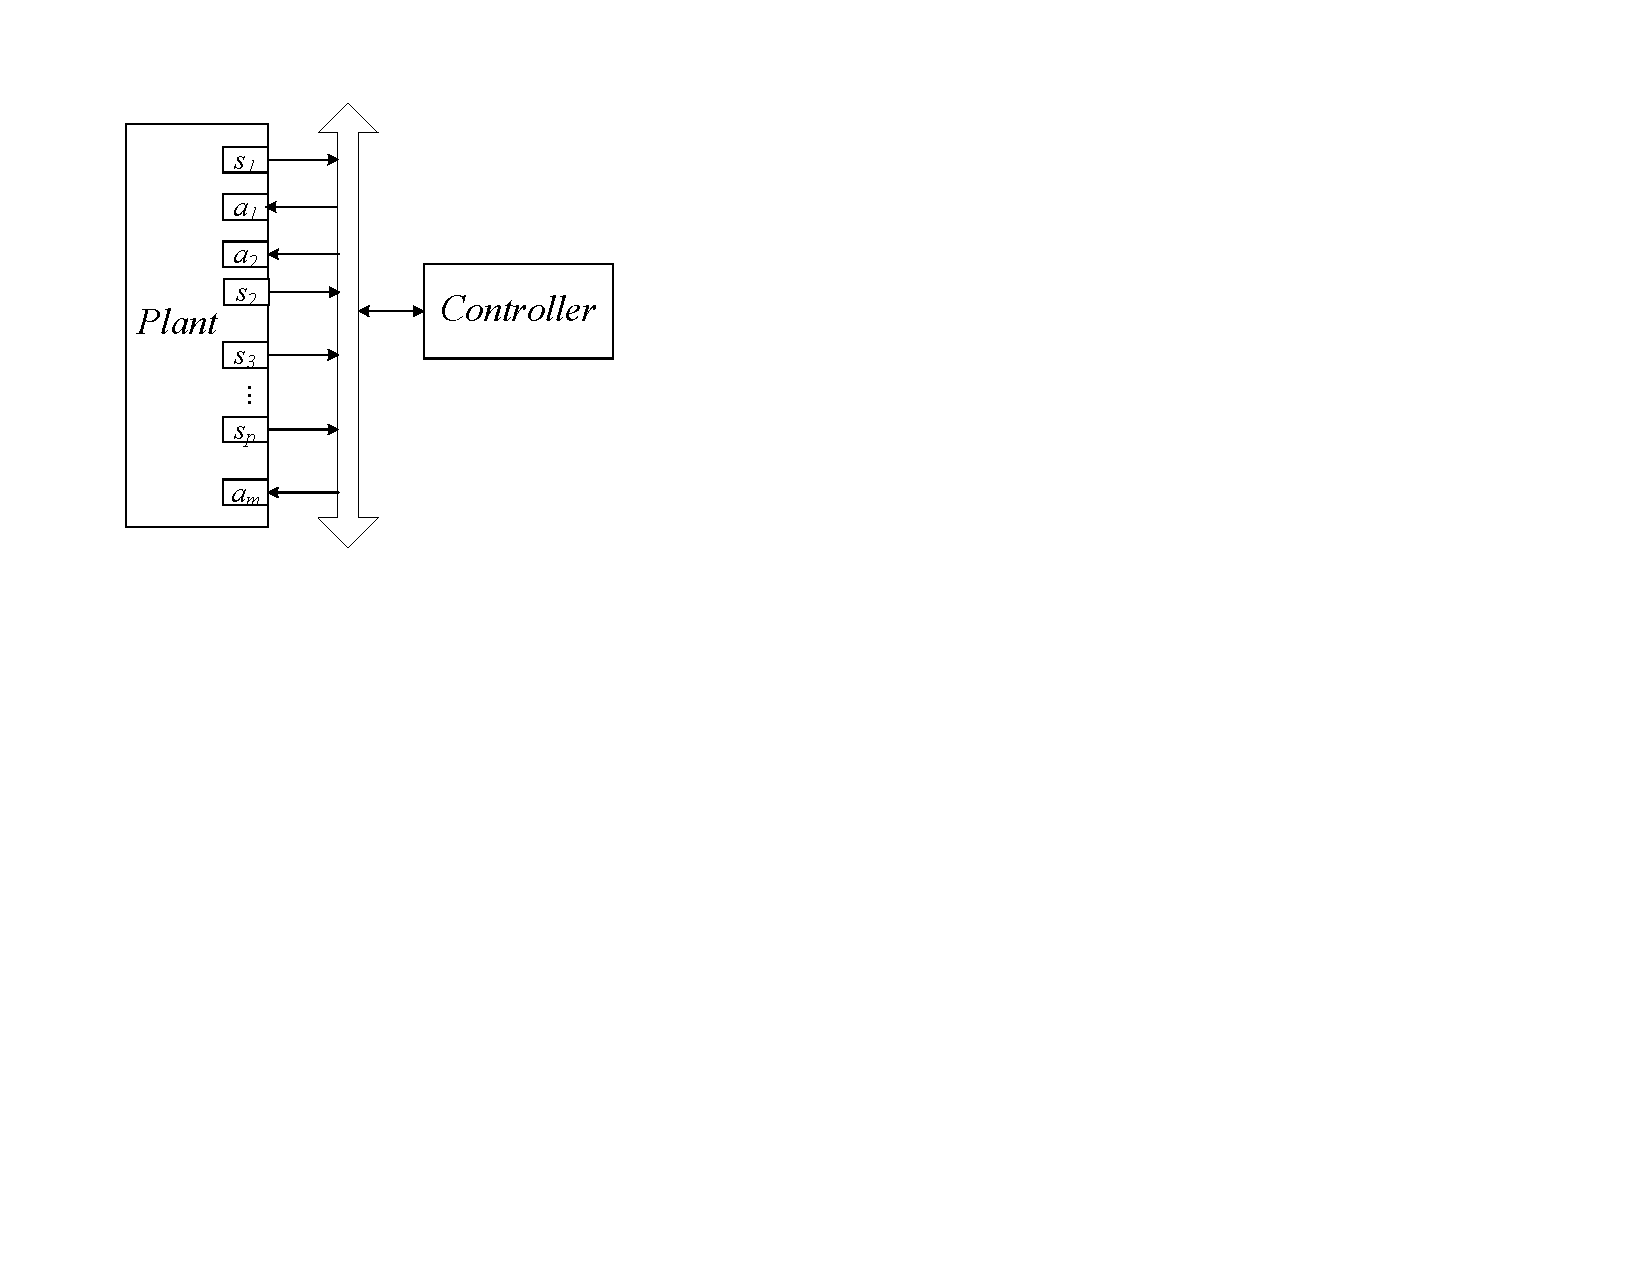
\includegraphics[width=0.24\textwidth]{figs/wired_system.pdf}
			\label{fig:System_wired}
		}	
	\subfigure [Wireless Network Controlled System] {
			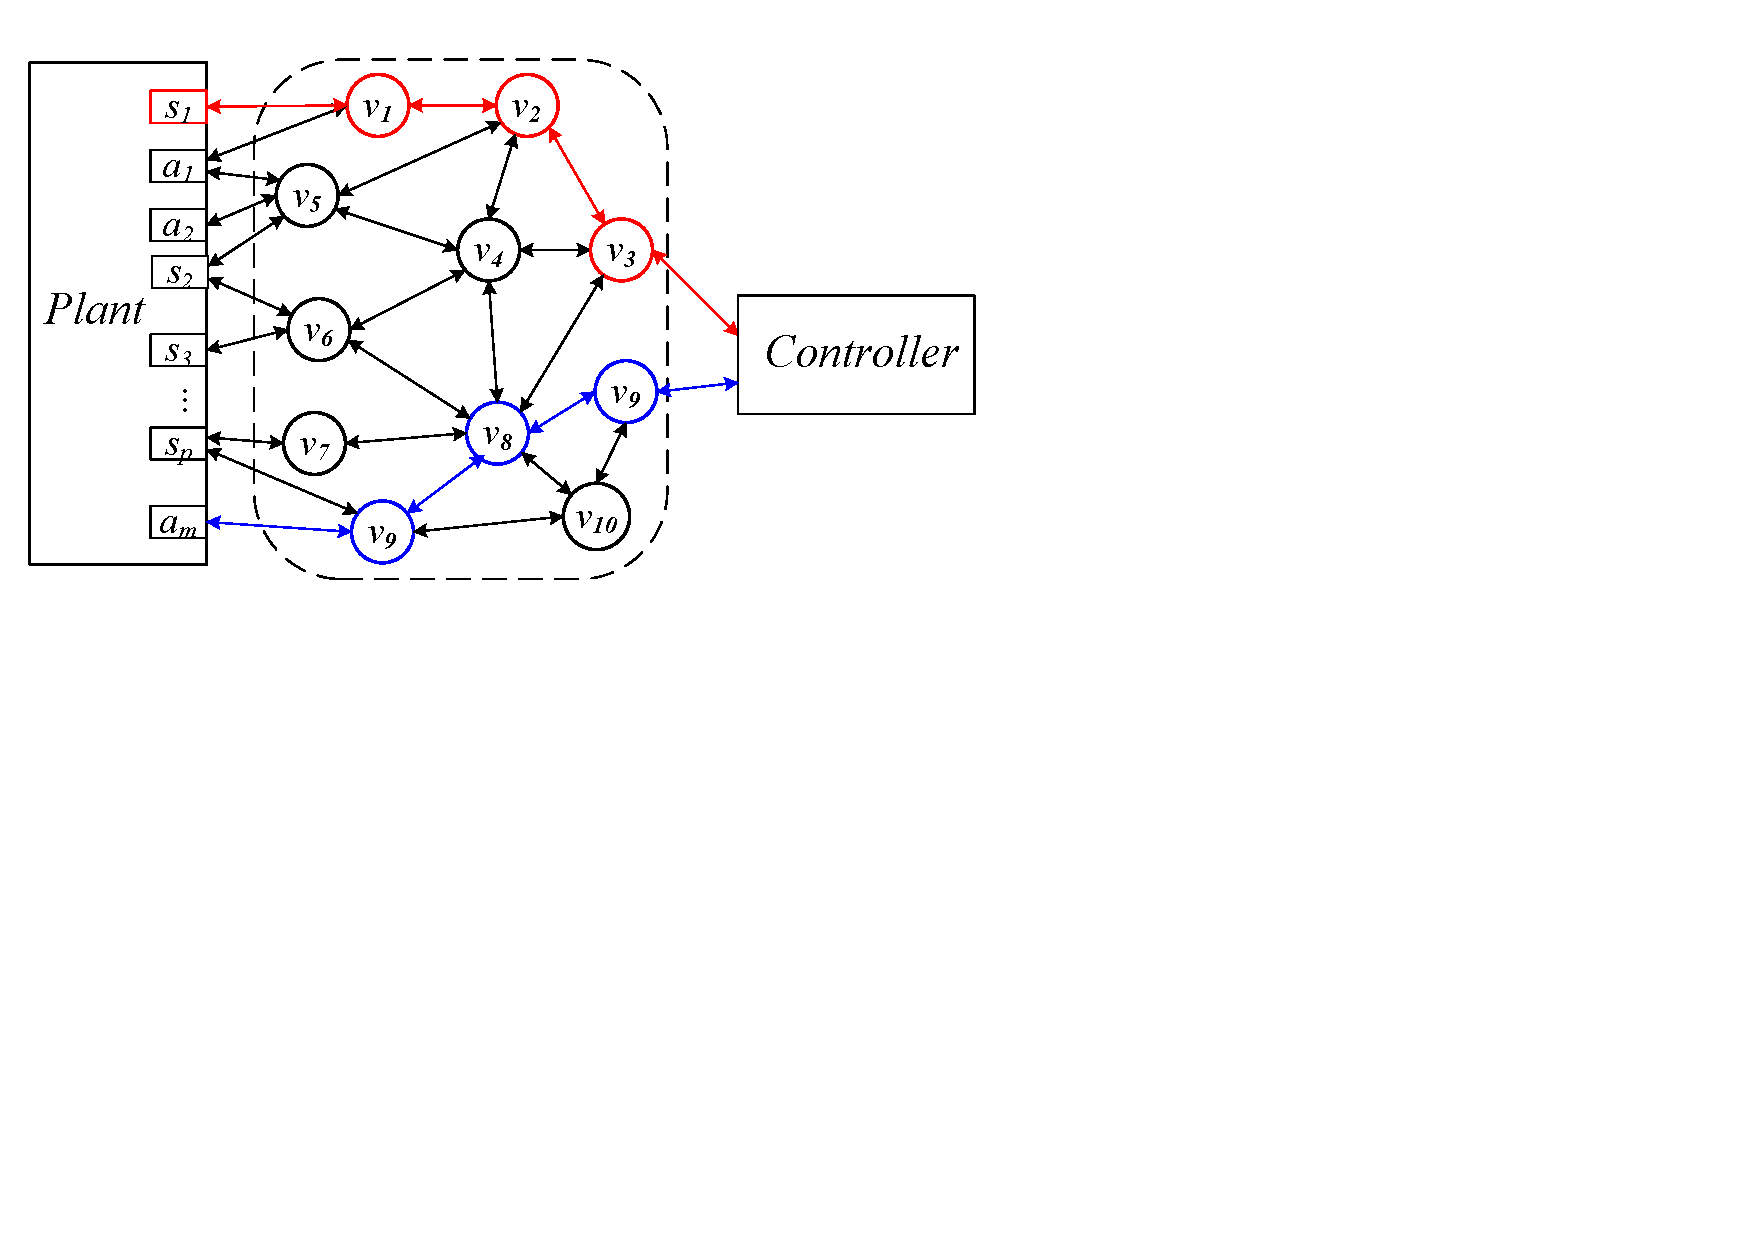
\includegraphics[width=0.37\textwidth]{figs/wcns_conv.pdf}
			\label{fig:wncs}
		}	
	\subfigure [Wireless Control Network] {
			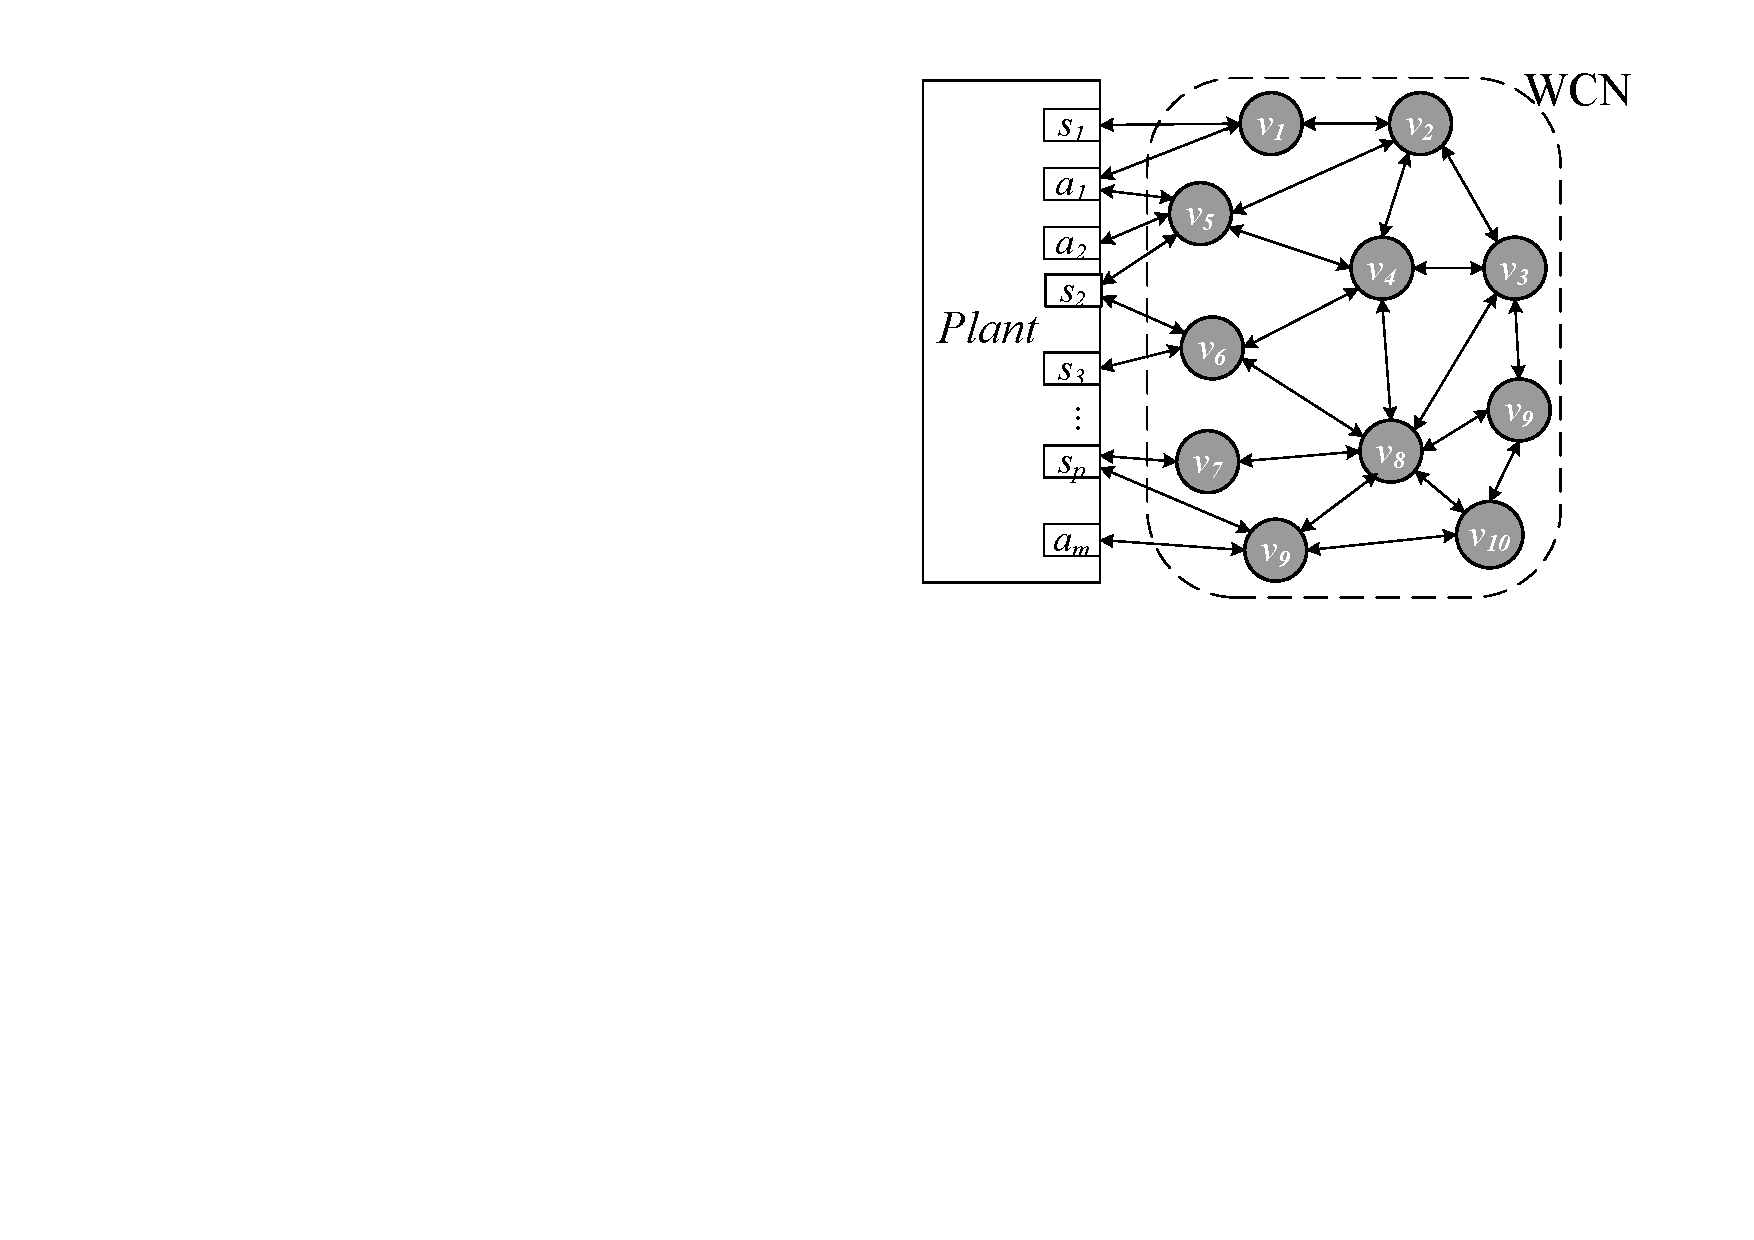
\includegraphics[width=0.28\textwidth]{figs/wcn_system.pdf}
			\label{fig:wcn}
		}	
	\end{center}	
\vspace{-10pt}
\label{fig:ncs_full}
\caption{Standard architectures for Networked Control Systems; (a) Wired system with a shared bus and dedicated controller; (b) Red links/nodes - routing data from the plant's sensors to the controller; Blue links/nodes - routing data from the controller to the plant's actuators; (c) A multi-hop wireless control network used as a distributed controller.}
%\vspace{-5pt}
\end{figure*}
%%%%%%%%%%%%%%%%%%%%%%%%%%%%%%%%%%%%%%%%%%%%%%%%%%%%%%
\textbf{3. DR Control Synthesis:}  While black-box and data-driven machine learning approaches are suitable for prediction, our primary contribution is making them capable of controller synthesis. 
Unlike rule-base DR, which does not account for building state and external factors, in DR synthesis the optimal control actions are derived based on the current state of the building, forecast of outside weather and electricity prices.
We introduce a novel model based control with regression trees (mbCRT) algorithm to enable control with regression trees for real-time DR synthesis. Using the mbCRT algorithm, we can optimally trade off thermal comfort inside the building against the amount of load curtailment. 
While regression trees are a popular choice for prediction based models, this is the first time regression tree based algorithms have been used for controller synthesis with applications in demand response. Our synthesis algorithm outperforms rule based DR strategy by $17\%$ (based on guidelines from Siemens) while maintaining bounds on thermal comfort inside the building.\vspace{4pt}

We have evaluated the performance of DR-Advisor using a mix of real data from 8 buildings (1.2 million square feet) on the campus of the University of Pennsylvania, a large office building in Philadelphia and data-sets from a virtual building test-bed for the Department of Energy's (DoE) large commercial reference building.
We also compared the performance of DR-Advisor against other data-driven methods using a bench-marking data-set from AHRAE's great energy predictor shootout challenge~\cite{kreider1994predicting} and rank second. The first place was achieved by the use of neural networks which are not interpretable, while DR-Advisor with regression trees is highly interpretable by facilities managers and provides them both guidance and provenance for decisions made to control their infrastructure.


\section{Closed-loop Control over Wireless Networks}
The current generation of embedded wireless systems has largely focused on open-loop sensing and monitoring applications. To address actuation in closed-loop wireless control systems there is a strong need to re-think the communication architectures and protocols for reliability, coordination and control \cite{wireless-ind}.  Wireless networked control systems, or Networked Cyber-Physical Systems (Networked-CPS),  fundamentally differ from standard distributed systems in that the dynamics of the \emph{network} (variable channel capacity, probabilistic connectivity, topological changes, node and link failures) can change the operating points and physical dynamics of the \emph{closed-loop system}~\cite{ncs_stability, ncs_survey}. The most important objective of control in Networked-CPS is to provide stability of the closed-loop system. It is therefore necessary for the network (along with its interfaces to sensors and actuators) to be able to provide some form of guarantee of the control system's stability in the face of the non-idealities of the wireless links and the communication constraints of the wireless swarm network. A secondary goal in Networked-CPS is to allow for composition of additional controllers and plants within the same network without requiring reconfiguration of the entire network operation.

The most common approach to incorporating Networked-CPS into the feedback loop is to use it primarily as a communication medium: the nodes in the network simply route information to and from one or more \emph{dedicated controllers}, which are usually specialized CPUs capable of performing computationally expensive procedures (see \figref{wncs}). The use of dedicated controllers imposes a routing requirement along one or more fixed paths through the network, which must meet the stability constraints, encapsulated by end-to-end delay requirements~\cite{chenyang, evm_rtas10}. 
However, this assignment of routes is a static setup, which commonly requires global reorganization for changes in the underlying topology, node population and wireless link capacities. 

Routing couples the communication, computation and control problems \cite{alur_tac11,sched_TTA_HART,sched_TTA_scal}. Therefore, when a new route is required due to topological changes, the computation and control configurations must also be recalculated. Merely inserting a WNCS into the standard network architecture ``sensor $\rightarrow$ channel $\rightarrow$ controller/estimator $\rightarrow$ channel $\rightarrow$ actuator'' requires the addition of significant software support~\cite{evm_rtas10, etherware},  as the overhead of completely recomputing the computation and control configurations, due to topological changes or packet drops, is too expensive and does not scale.

 %%%%%%%%%%%%%%%%%%%%%%%%%%%%%%%%%%%%%%%%%%%%%%%%%%%%%%
\begin{figure*}[!t]
	\begin{center}
	`	\vspace{-5pt}
	\subfigure {%[\small (a) A wireless sensor, actuator and controller network. (b) Algorithm assignment to a set of controllers, each mapped to the respective nodes. (c) Three Virtual Components, each composed of several network elements.] {
	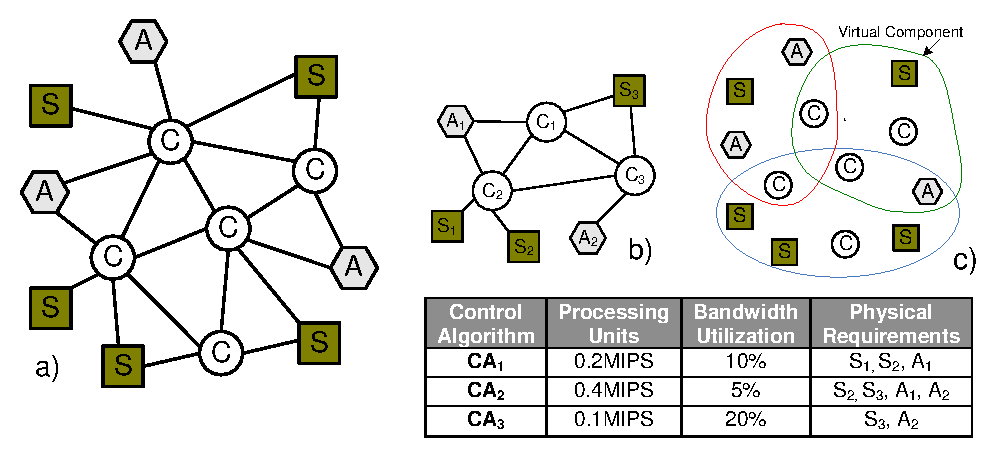
\includegraphics[width=0.55\textwidth]{figs/component_new.eps} 
  \vspace{-5pt}
	%\caption{\small (a) A wireless sensor, actuator and controller network. (b) Algorithm assignment to a set of controllers, each mapped to the respective nodes. (c) Three Virtual Components, each composed of several network elements.}
	\label{fig:component}
	}
	\hspace{.1in}
	\subfigure {%[(d) \small Decoupled virtual tasks and physical nodes with runtime task mapping.] {	
			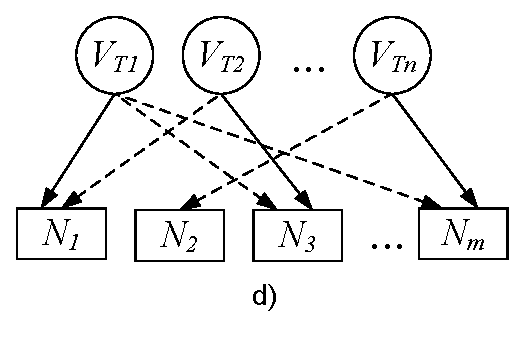
\includegraphics[width=0.3\textwidth]{figs/taskmap.eps}
			\label{fig:taskmap}
		}
	\end{center}	
\vspace{-15pt}
\caption{(a) A wireless sensor, actuator and controller network. (b) Algorithm assignment to a set of controllers, each mapped to the respective nodes. (c) Three Virtual Components, each composed of several network elements. (d) Decoupled virtual tasks and physical nodes with runtime task mapping.}
\label{fig:overview}
\vspace{-5pt}
\end{figure*}
%%%%%%%%%%%%%%%%%%%%%%%%%%%%%%%%%%%%%%%%%%%%%%%%%%%%%%

While providing a review of classical and recent approaches for control over wireless networks, we present two complementary approaches on maintaining stability in the presence of environment and network disturbances. The first approach adopts a ``computer systems" perspective on the design of robust architectures for embedded wireless control and actuation. We call this scheme Embedded Virtual Machines (see \figref{overview}) which provides software mechanisms to decouple controller functionality from the physical node - thus providing resilience to node, link and topology changes. The second approach adopts a ``control theoretic" perspective on distributed control within the network (see \figref{wcn}). This provides control mechanisms to remove controller functionality from a dedicated node to all nodes in the network - thus eliminating the need for routing and guaranteeing stability and optimal control in the presence of link, node and topology changes. 

\subsection{\textbf{Embedded Virtual Machines}}
Current approaches for robust networked control%algorithms
~\cite{ncs_survey} require the underlying network to satisfy a minimal set of requirements (e.g. guaranteed packet deliver rate, upper bound on network induced delay) and reduce the network model to that of a single channel with random delays. In addition, they do not address the spatial aspects of the network, i.e., how changes in the network topology affect the closed-loop system performance.

As the links, nodes and topology of wireless systems are inherently unreliable, such time-critical and safety-critical applications require programming abstractions where the tasks are assigned to the sensors, actuators and controllers as a \emph{single component}, rather than statically mapping a set of tasks to a specific physical node at design time (as shown in \figref{overview}). Such wireless controller grids are composed of many nodes that share a common sense of the control application but without regard to physical node boundaries. Our approach, is to \emph{decouple} the functionality (i.e., tasks) from the inherently unreliable physical substrate (i.e., nodes) and allow tasks to migrate/adapt (\figref{overview}(d)) to changes in the topology. 

To this end, we introduced the Embedded Virtual Machine (EVM), a powerful and flexible programming abstraction where a Virtual Component (VC) and its properties are maintained across node boundaries~\cite{evm_rtas10,evm_tecs11}, as shown in Fig. 2(c). EVMs differ from classical system virtual machines. In the enterprise or on PCs, one (powerful) physical machine may be partitioned to host multiple virtual machines for higher resource utilization. On the other hand, in the embedded domain, an EVM is composed across multiple physical nodes with the goal to maintain correct and high-fidelity operation even under changes in the physical composition of the network. The goal of the EVM is to maintain a set of \emph{functional invariants}, such as a control law and \emph{para-functional invariants} such as timeliness constraints, fault tolerance and safety standards across a set of controllers given the spatio-temporal changes in the physical network. Thus, the EVM introduces new degrees of freedom, task migration and routing which facilitates, at runtime, the network configuration (operating point, conditions) to meet the requirements of the networked control algorithms. However, the EVM does not provide explicit guarantees but only finds the optimal operation configuration in terms of routing and task assignment.

\subsection{\textbf{Distributed Control over Wireless Networks}}
Let us consider the problem of stabilizing a plant with a multi-hop network of resource constrained wireless nodes. 
In ~\cite{wcn_tac11}, we introduced the concept of a {\it Wireless Control Network} (WCN), which is a paradigm change for distributed control over a wireless network. In a WCN the entire network {\it itself} acts as a controller, as the computation is spread over the whole network, instead of assigning a particular node with the execution of the control procedure.  We have devised a numerical design procedure that produces the coefficients of the linear combinations for each node and actuator to apply in order to stabilize the plant.  The radio connectivity between nodes in the network induces topological constraints to the control algorithm, and this topology determines whether it is even possible to stabilize the system with the use of linear iterative strategies.  In addition, a method to synthesize an optimal WCN, with respect to the standard cost functions, has been developed~\cite{JIISc_distrCPS}. 

Given the fundamental unreliability of wireless communication, the WCN method handles topological constraints while maintaining mean square stability for packet drop rates \textbf{\emph{up to 20\%}} for a specific network topology and plant. This bridges the gap between the basic WCN and the theoretical upper bound of robustness to packet drops~\cite{Hadjicostis02}. We also show a method to synthesize a WCN robust to a certain level of node failures, and then extend the synthesis procedures to allow for the use of the WCN for control of continuous-time plants. 

While in the past efforts, we consider scenarios where the network topology is already set, in recent efforts~\cite{wcn_jsac12, wcn_cdc11} we have investigated a dual problem, ``how to synthesize the network so that a stable WCN configuration exists?" The topological conditions from~\cite{wcn_jsac12}, along with the results from~\cite{wcn_tac11} provide the essential building blocks for an integrated decentralized wireless control network design framework. Early experiments in an industrial process control case study of a distillation column in a process-in-the-loop test-bed demonstrate optimal control of continuous-time physical processes which maintain system stability under the presence of node and link failures. 

\subsubsection{Advantages of the WCN}
The WCN introduces very low communication and computation overhead. The linear iterative runtime procedure is computationally very inexpensive as each node only computes a linear combination of its value and values of its neighbors. This makes it suitable for resource constrained, low-power wireless nodes (e.g., Tmote).
Furthermore, the communication overhead is also very small, as each node needs to transmit only its own state once per frame.  In the case when a node maintains a scalar state it transmits only \emph{2 bytes} in each message, making it suitable to combine this scheme with periodic message transmissions in existing wireless systems. 

The WCN utilizes a simple transmission schedule where each node is active only once during a TDMA cycle and the control-loop does not impose end-to-end delay requirements. This allows the network operator to decouple the computation schedule from the communication schedule, which significantly simplifies closed-loop system design and enables compositional design and analysis. 
 \section{Verification of Autonomous Vehicle Planning}

\begin{figure*}
	\centering
	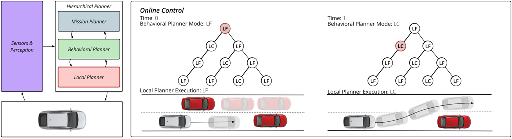
\includegraphics[width=1.8\columnwidth]{Figures/apex_stack}
	\caption{Autonomous vehicle planning stack with a behavioral planner which continually makes decisions. For example, when the decision to change lanes is made, the local planner must find a safe and smooth trajectory to follow around dynamic obstacles whose behavior is not fully known.}
\label{fig:apex_stack}
\vspace{-10pt}
\end{figure*}

  Each year there are an average of 1.24 million traffic fatalities around the world \cite{Waldrop2015}. Estimates indicate that more than 90 percent of all accidents are due to driver error \cite{Waldrop2015}. Competent autonomous vehicles (AVs) could drastically reduce the occurrence of such incidents, but a major question first needs be answered:
  how can we judge when an AV is ready to graduate from research laboratories to public roads?
  One thing is clear: the public will want significant evidence that AVs are indeed safe \cite{weld1994first}. 
  This raises significant ethical and legal questions about how the AV should behave, and technical questions about how to \emph{verify} that it will always behave the way its designers intended.\vspace{4pt}
  
\emph{How do you give a self-driving car a driver's license?}\vspace{4pt}

~Prototype AVs have driven millions of miles and are even being approved for \emph{testing} on public roads in some states \cite{Iozzio2014}; however, manufacturers cannot \emph{verify} (i.e., guarantee) the safety of even the simplest of scenarios in the presence of other dynamic traffic participants. 
  Compounding, the difficultly of vehicle certification, vehicle manufacturers such as Tesla are transitioning to frequent over-the-air software updates. Such practice eschews conventional vehicle development technique and greatly increases pressure on developers to deliver correct software at a rapid pace. 
 
  The net result of the growing pressure to release AVs is a wide gap between current regulations and our technological capabilities. 
  Human drivers are not `certified' to act safely in all situations, in fact, we know they don't; however, they assume liability for their actions.
  Who is liable for the behavior of an AV? 
  Currently, it appears that manufacturers will take one of two approaches: (1) assume liability for the actions of the vehicle and self-insure \cite{volvo15Liability} or (2) force the human occupants of an AV to make all critical decisions and shift liability to the pilot \cite{maurer2015autonomes}. In either case, even if AVs reduce accidents by 99 percent, it is likely that the 1 percent of remaining accidents will invariably spawn a myriad of legal actions against \emph{both} manufacturers \cite{russell2015research} and vehicle owners.   
  If the legal question is not answered, these risks could stifle the development of the AV market.
  
    \begin{figure}[!b]
    	\centering
	\vspace{-10pt}
	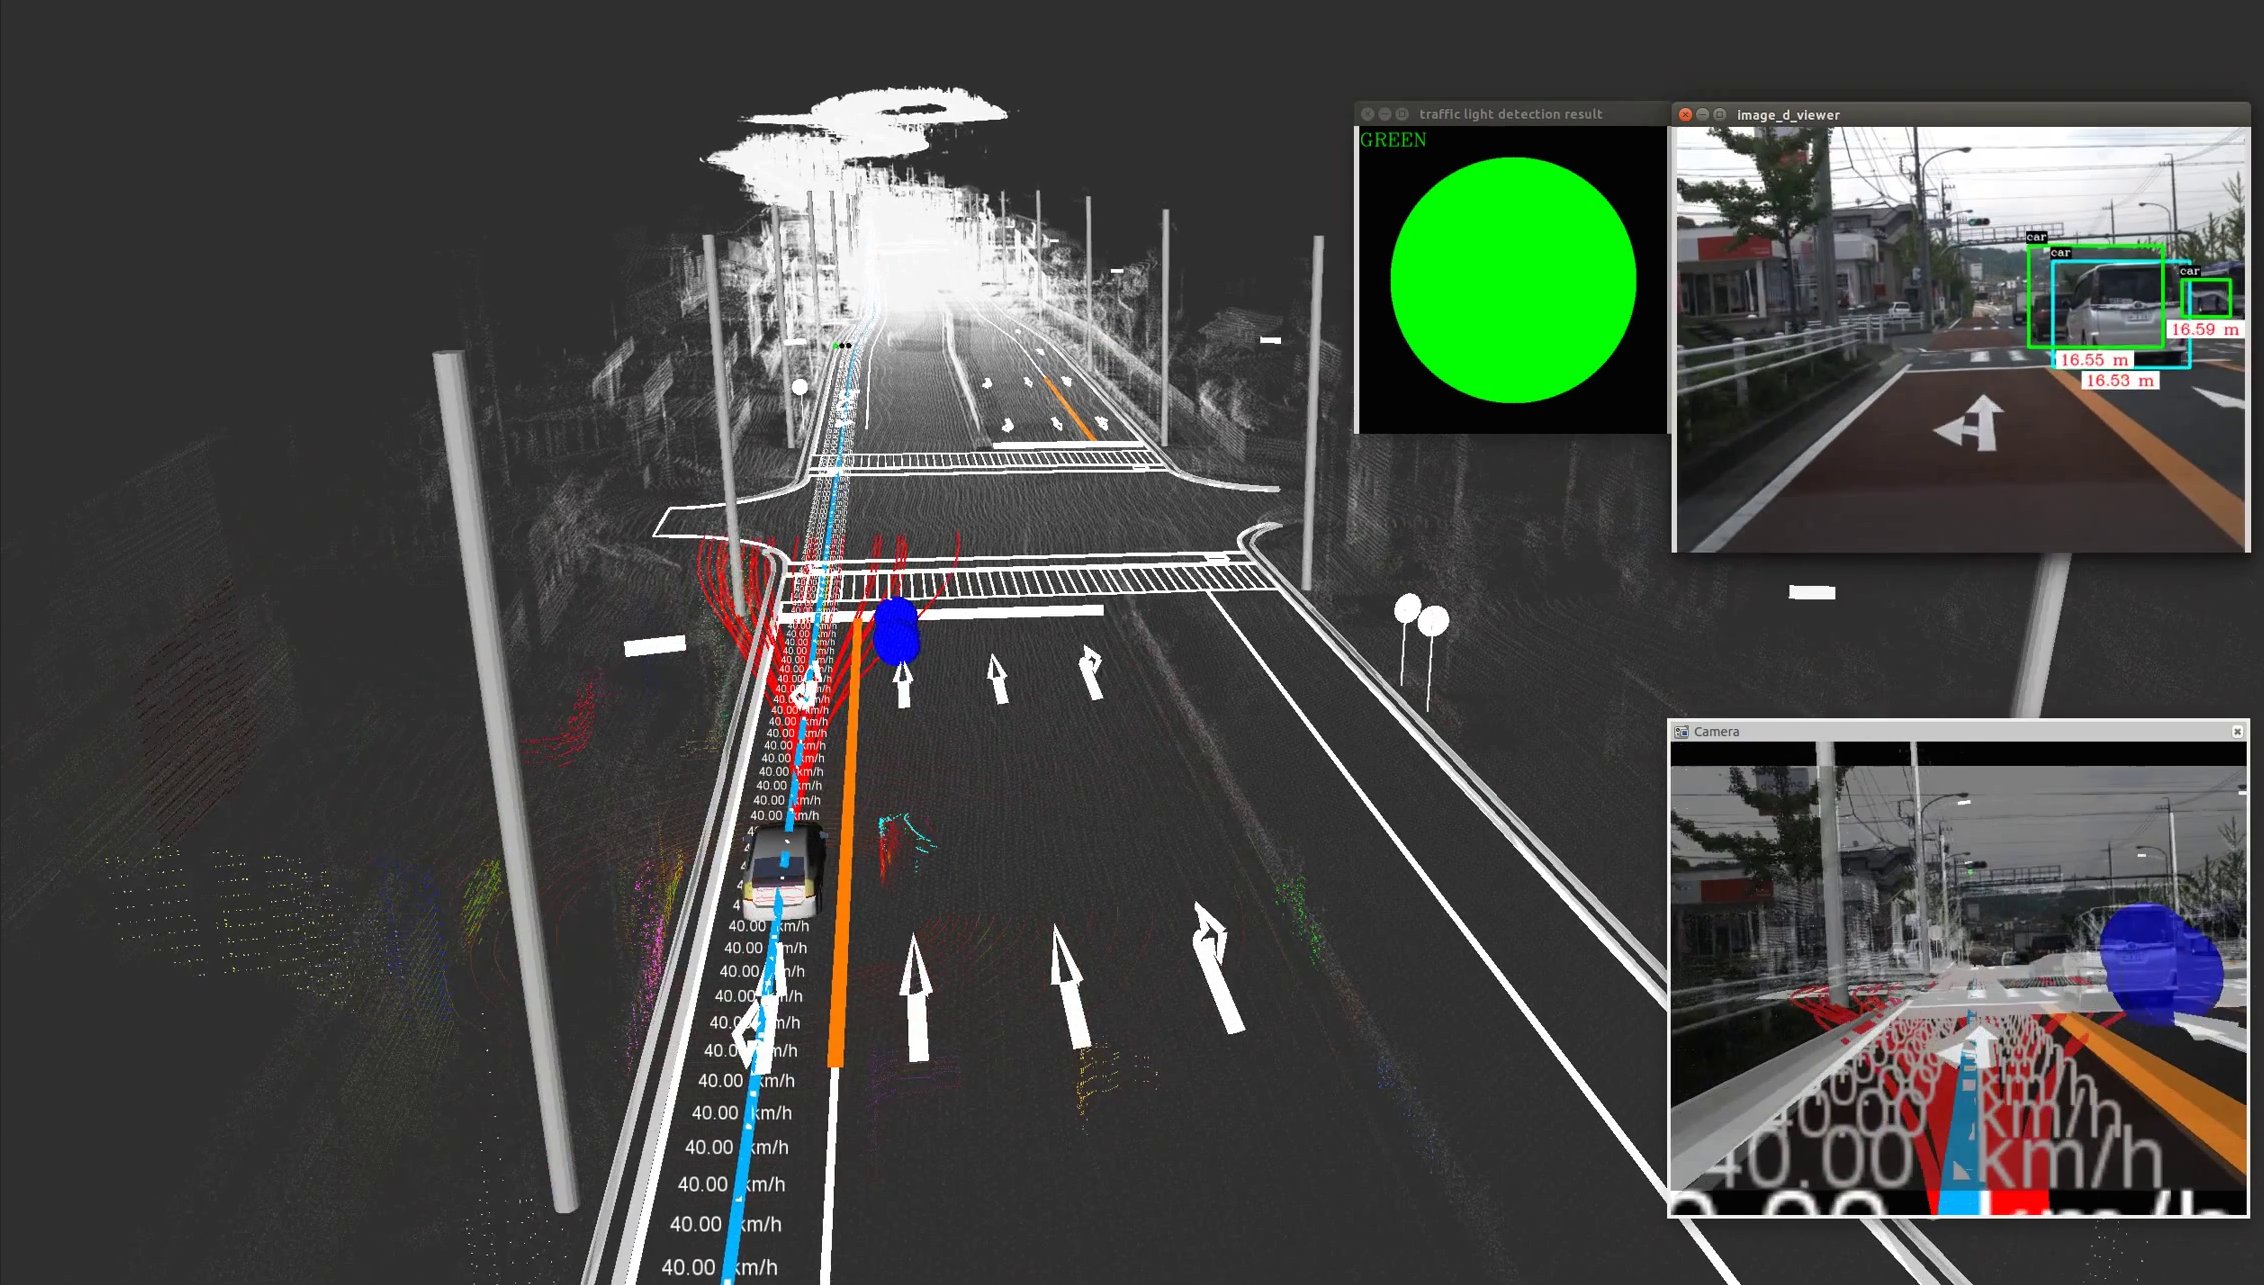
\includegraphics[width=\columnwidth]{figures/apex_planning.png}
	\caption{Autonomous vehicle with LiDAR, camera and map data.}
	\label{fig:apex_planning}
\end{figure}

  Thus, regardless of where legal liability falls it is clear that we first need new, practical methods for verification and validation of the decision engines of each AV (as shown in \figref{apex_stack}).
  Furthermore, verification must be automatic, exhaustive, and expedient for clearly defined scenarios. 
  Secondly, ethical considerations still underlie both the design and verification of AVs: how does the safety of the car's passengers weigh against that of people in its environment? 
  Whose morals are embedded in the decision engines of an AV?
  
 \subsection{New and Old Challenges}
 There are several fundamental safety challenges in verifying and implementing autonomous vehicles, including:
\begin{enumerate}
\item As shown in \figref{apex_planning}, in a given driving scenario, the vehicle�s planning controller must determine all possible pathways in the road and provide the supervisory controller with the safest trajectory while interacting with other agents (vehicles, pedestrians, bicyclists), obeying flow control infrastructure (stop signs, traffic lights, environment conditions) and adhering to traffic rules;
\item While the target vehicle is controllable, the state evolutions of other agents are uncertain and the target vehicle must continuously adapt its plan as the scenario evolves;
\item At any time, the driver may interject to take over control of the vehicle.
\end{enumerate}
 
Some of the problems facing would-be AV manufacturers in 2016 are very different than those outlined by the teams in the 2007 DARPA Urban Challenge \cite{buehler2009darpa}. One problem highlighted by the first ever crash between AVs at the Urban Challenge \cite{fletcher2008cornell} is that there are no known \quotes{formal methods that would allow definitive statements about the completeness or correctness of a vehicle interacting with a static environment, much less a dynamic one} \cite{urmson2008autonomous}.  Today one must still consider the massive configuration space of each individual snapshot of the day-to-day life of an AV if verification is to be attempted. For example, in order to test the interaction between two 7 DOF AVs requires $10^{14}$ simulations for only 10 samples from each state. If each test takes 10 seconds, the resulting set of simulations will take \emph{30 million years} to complete. Furthermore, within a given scenario, errors in localization, sensing, and actuation imply we never know the state of the world exactly. Small state estimation errors can befuddle motion planning algorithms and mean a difference between collision and safety in tight spots. As many teams in the Urban Challenge noted, a means of verifying the safety of autonomous driving is paramount to putting self-driving cars in the hands of the public \cite{urmson2008autonomous}. 

%% In contrast to the Urban Challenge in 2007, in which only 6 teams out of an original 89 applicants were able to finish, many research labs find themselves in the position of being able to construct a convincing AV in a matter of months; such a vehicle might be relatively competent in 75 percent of the situations it faces, but the long tail of special cases beckons. In fact Sebastian Thrun, a veteran of Google's Self Driving Car project and the Urban Challenge, notes that \emph{there were many more of unusual situations than we believed in the beginning}. One possible solution to handling rare events and scenarios is to record such occurrences using consumer vehicles driving in real traffic; with each new scenario existing behavioral planners can be adjusted via a reinforcement learning scheme \cite{wei2013autonomous, Silver_2010, Waldrop2015}. Just as in the more vanilla scenarios, timely updates to controllers provided on the basis of a single example will need to be verified offline, before shipping, and without the thousands of miles of testing necessary for a typical safety feature. 



%As Brian Soublet of the California DMV pointed out, he knows how to test a 16-year-old's driving skills, but he can't say the same for a car. At the same time, these regulators know that when a death inevitably happens—no amount of %self-driving cars will reduce annual road deaths to zero—they'll be attacked for allowing unsafe vehicles on the road.
\begin{figure}[b]
	\centering
	\vspace{-10pt}
	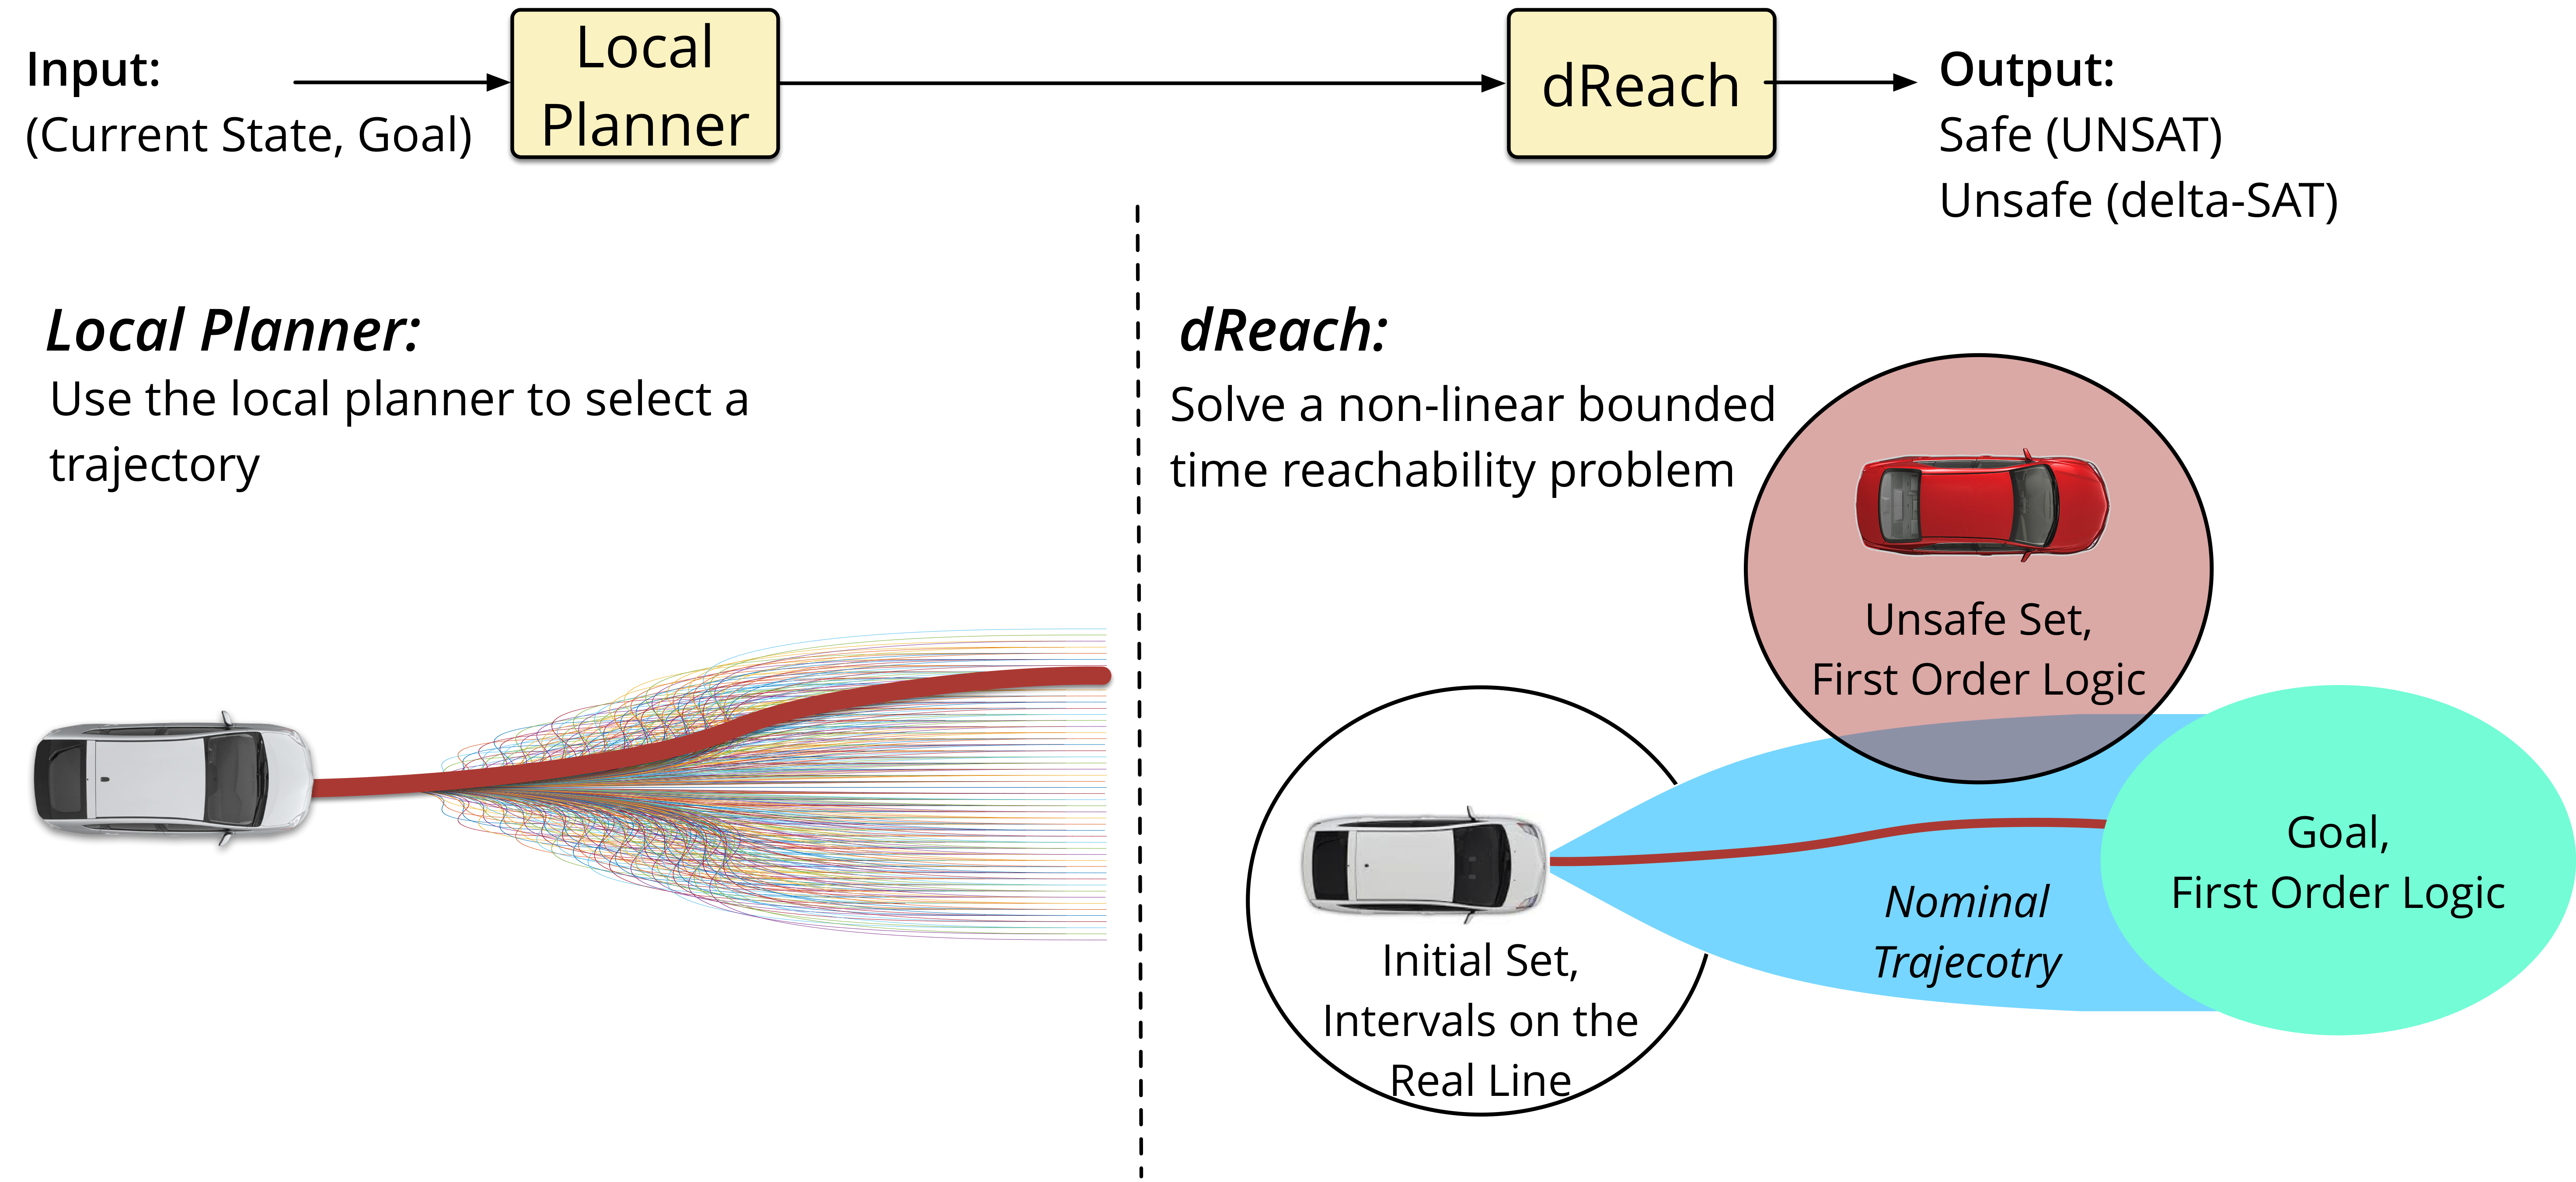
\includegraphics[width=\columnwidth]{Figures/tool_single}
	\caption{A single offline execution of the APEX tool calls the local planner associated with the AV in order to generate a reachability problem}
	\label{fig:apex_tool}
\end{figure}

\subsection{APEX: Autonomous vehicle Plan verification \& EXecution}
The APEX tool represents a new approach to solving both the problems of the Urban Challenge and investigating rare events encountered only through on road driving and testing. Unlike other tools capable of verifying controllers for hybrid systems we require almost no abstraction. Most current approaches look at only the behavioral layer and assume perfect implementation of plans at the motion planning layer. Instead, as shown in \figref{apex_tool}, we propose that the behavioral layer is used to generate sequences of problems to be investigated at the level of motion planning and trajectory tracking.  Thus, APEX addresses the safety verification issue by leveraging new results in hybrid systems and reachability analysis \cite{gao2013satisfiability} to convert a brute force search over real intervals (which is intractable) into a set of finite sequences of bounded reachability problems. 

With APEX, we capture the output of trajectory generation and optimization based methods outside of the formal model of the system. Using such information, we generate a sequence of verification problems by running the trajectory through realistic vehicle dynamics and low level controls. The software which runs on the vehicle is used directly for verification with the Robot Operating System (ROS). If a rare event is encountered and recorded by a real vehicle and a new rule or controller is added to the AV it is imperative that the manufacturer have high confidence that the modification will not induce new errors which are not evident in a single trace. APEX can make the most of rare events and scenarios; given a template we could find every possible instantiation and prove it is impossible for solution to make a decision leading to crash. 

The key features of our approach are: (1) Use of realistic planning software which runs on actual vehicles. (2) Modular vehicle model construction which can easily be replaced when new algorithms or alternate vehicle dynamics are necessary. (3) Non-conservative evaluation of safety and liveness at the level of the ego-vehicles actual spatial-temporal evolution. 

Thus, verification of realistic scenarios under all possible configurations over a length of 30-60 seconds is entirely feasible. Using such an approach a manufacturer, regulator, or insurer can begin to build a library of scenarios on which to test new vehicle software or updates made to the behavioral layer made through a reinforcement learner.
 
 \subsection{Open Challenges for Autonomous Vehicle Safety}
\noindent\textbf{1. Scenario Composition for Safe Journeys}

Safety certification will seek to verify that a complete mission, made up of several independently verified scenarios, can be composed to ensure the safety across a journey (i.e. sequence of scenarios). The greatest challenge will be ensuring that the transitions between scenarios will result in safe initial conditions. As not all interactions are observable or captured in formal models, work also needs to be performed on the integration of informal assurance case arguments in a structured manner within APEX. This will also assist in evaluating cooperative and collaborative interactions with the human-in-the-loop.\vspace{0.4pt}

\noindent\textbf{2. Conformance-based Controller testing within the scenario context}

A framework for black-box conformance testing of autonomous vehicle controllers within the context of one or more scenarios is essential for the creation of high confidence code from verified systems and scenarios.\vspace{0.4pt}

\noindent\textbf{3. Property hierarchy for unrealizable specifications}

When a human operator is faced with an unrealizable specification it is common for the driver to knowingly violate a lesser priority safety property i.e. the driver may swerve on to the shoulder lane to avoid a sudden braking vehicle in front. In the context of autonomous driving in general, one can consider that many unrealizable scenarios might arise due to the initialization of the environment. Thus, for each scenario we need to assign priorities to properties such that lower priority properties may be violated to ensure higher priority properties are maintained under extreme scenarios.  
%% \subsection{Verification, learning, ethics, and control}
%In the literature on robot ethics, it remains arguable whether artificial agents without free
%will can truly exhibit moral behavior [1]. However, it seems certain that other road users
%and society will interpret the actions of automated vehicles and the priorities placed by their
%programmers through an ethical lens. Whether in a court of law or the court of public opinion,
%the control algorithms that determine the actions of automated vehicles will be subject
%to close scrutiny after the fact if they result in injury or damage. In a less dramatic, if no
%less important, manner, the way these vehicles move through the social interactions that
%define traffic on a daily basis will strongly influence their societal acceptance. This places
%a considerable responsibility on the programmers of automated vehicles to ensure their
%control algorithms collectively produce actions that are legally and ethically acceptable to
%humans.
		 %\begin{itemize}
		 %	\item Trolley problem
		 %	\begin{itemize}
		 %		\item Level of semantic detail and embellishment added to such scenarios is unrealistic.
		 %		\item The first vehicles to market will simply be programmed with a concept of forward safety.
		 %		\item No manufacturer will ever program an autonomous vehicle to swerve into another vehicle. The pretense of such problems is ridiculous.
		 %		\item Trolley problem does not have a correct solution, instead we should be asking how can we prove that \emph{trolley problems cannot occur based on decisions made by an autonomous agent}
		 %	\end{itemize}
		 %\end{itemize}
 
%% The likely arrival of learned behaviors and the accompanying cost functions which allow the discrimination between multiple feasible strategies will necessitate careful consideration regarding the quantification of desireable robot behaviors. It is easy to personify the \emph{software agent} which operates an AV; naturally, this leads to the consideration of such an agent's ethical duties. It is not clear whether such software can truly exhibit ethical behavior or rather simply mimic the instructions of the designer. Nevertheless, \quotes{it seems certain that other road users and society will interpret the actions of automated vehicles and the priorities placed by their programmers through an ethical lens} \cite{maurer2015autonomes}. In order to improve the safety, efficacy, and percieved morals of AVs we propose 3 areas of promising future research: 
%% \begin{itemize}
%%	 \item Automatic verification of learned behaviors and cost functions
%%	 \item Hierarchical property satisfaction and instantiation of temporal logic constraints in a model predictive control framework
%%	 \item Online verification of behavioral plans \cite{wei2014behavioral} over a range of 5-10 seconds
%% \end{itemize}
 

%% We have already argued that verification of learned behaviors and cost functions is necessary; we propose that such activities should be fully \emph{automated} in manner similar to static verification of source code. Before an update is released it will be subjected to an ever increasing battery of common verification scenarios. Secondly, we intuit that describing vehicle actions as ethical implies that there exists a ranking function over potential behaviors; if vehicle specifications are described hierarchically we can actually dictate and examine the ethics of a particular AV. For example, it may be desirable that only in a near crash situation the AV disregards the speed limit and lane keeping behaviors in order to avoid an accident. Finally, we propose that such \emph{offline} verification techniques in APEX be reimagined and refactored for short-horizon online verification of all potential vehicle actions. It is likely that initial forays into autonomy may require handoffs between human and machine. Studies show \cite{blanco2013human} that a safe handoff requires 5-8 seconds of preparation. Thus, online verification techniques may be used to discover potential system failures and provide fair warning to the driver. 
\section{Co-design of Computation and Control for Autonomous Systems}
\subsection{Motivation}

Real-time control of autonomous vehicles requires the processing of a large amount of sensor data from cameras, LIDAR, radars, encoders, inertial sensors and possibly information communicated by other vehicles or the road infrastructure.
This data is used by the vehicle to determine its position in the world and that of neighboring obstacles, which we refer to as \emph{state estimation}, and to calculate its next move.
Google's autonomous vehicles generate over 750MB/s of sensor data \cite{diamandis2015bold} which must be processed by the perception pipeline fast enough for timely control decisions.
The perception pipeline uses \emph{run-to-completion} algorithms: such algorithms must always meet a pre-defined termination criterion before returning a useful answer.
If interrupted early, they don't return anything useful to the controllers.
Typical algorithms in a perception pipeline span tasks like edge detection, filtering, segmentation, object recognition and tracking, and sensor fusion. 
 
Perception algorithms have variable execution times because their runtimes depend on the current context.
E.g., a corner detector will take longer to detect all the corners in a rich scene than in a flat homogeneous scene (at a given processor frequency).
Because of this variability, the hardware running these run-to-completion algorithms is over-engineered for the worst-case execution time.
That is, the system is equipped with hardware that can always execute the software within a certain deadline.
When the current context causes the perception pipeline to perform the most operations (e.g., the corner detector has to find many corners), this is appropriate.
However, such worst-case situation rarely holds in practice. 
The rest of the time, the perception pipeline has fewer operations to perform within the deadline, so a slower (and less power-hungry) hardware execution would be appropriate.
The downside with this over-engineering is unnecessarily large power consumption for the average case.
For example, in many research autonomous vehicles, this leads to a requirement of up to 4KW in computational power \cite{powerNagoya}. 
This is a significant drain on the vehicle's lithium-ion battery capacity, which is 24kWh in a Nissan Leaf, for example.
It is also a significant compared to the average power drawn by the drive motors, which is around 3KW in a small electric vehicle modeled in ADVISOR \cite{nreladvisor} going through the Urban Dynamometer Drive Cycle. 
%%\mynote{HA}{30kW is peak, no?}
%%\mynote{YP}{Yes, good point, corrected. Also changed over 4KW to upto 4KW, don't want to claim too much esp. since we do not have concrete data on it. And please check the private communication citation for it.}

In addition to the high power consumption, the rigid nature of the run-to-completion algorithms used for perception and state estimation restricts the range of maneuvers that autonomous systems can do, e.g. autonomous cars are not yet capable of fast or aggressive driving.
Reacting faster to a dynamic scene requires a perception pipeline (and state estimation) that can deliver answers faster, even if the cost is slightly worsened quality of output.

\subsection{Challenge}
The challenge is to enable less power-hungry autonomous vehicles that still maintain the \emph{control performance} of current systems.
Note that the emphasis is on control performance, and not on the output quality of the perception algorithm.
While in general, the two are positively correlated (better output quality means better control performance) there are situations where this is not the case.
For example, if the lower quality output is produced faster, allowing a faster update of the control input.

From the above discussion it can be seen that we ought to design control algorithms that recognize how soon an update is needed from the perception and state estimation (P\&SE) pipeline. 
Correspondingly, we should also design P\&SE  algorithms that can provide useful answers even when interrupted before their run-to-completion criterion has been met. 
The main challenges in such a system are:
\begin{itemize}
\item Enabling common perception algorithms to provide useful (if lower quality) answers early.
This is a challenging task for any given algorithm as they are most often designed and implemented for maximum performance without consideration for the possibility of interruption.
\item Development of control/scheduling algorithms that are aware of when to request faster updates for the optimal operation of the closed loop system.
Existing work models the effect of delays on control and designs controllers that operate well despite the delay.
Here we are suggesting that rather than view the delays as purely adversarial, the controller should be aware of the range of trade-offs afforded it by the P\&SE algorithms and exploit these trade-offs for lower-power control. 
\end{itemize}
\begin{figure}[!b]
	\centering
	\vspace{-20pt}
	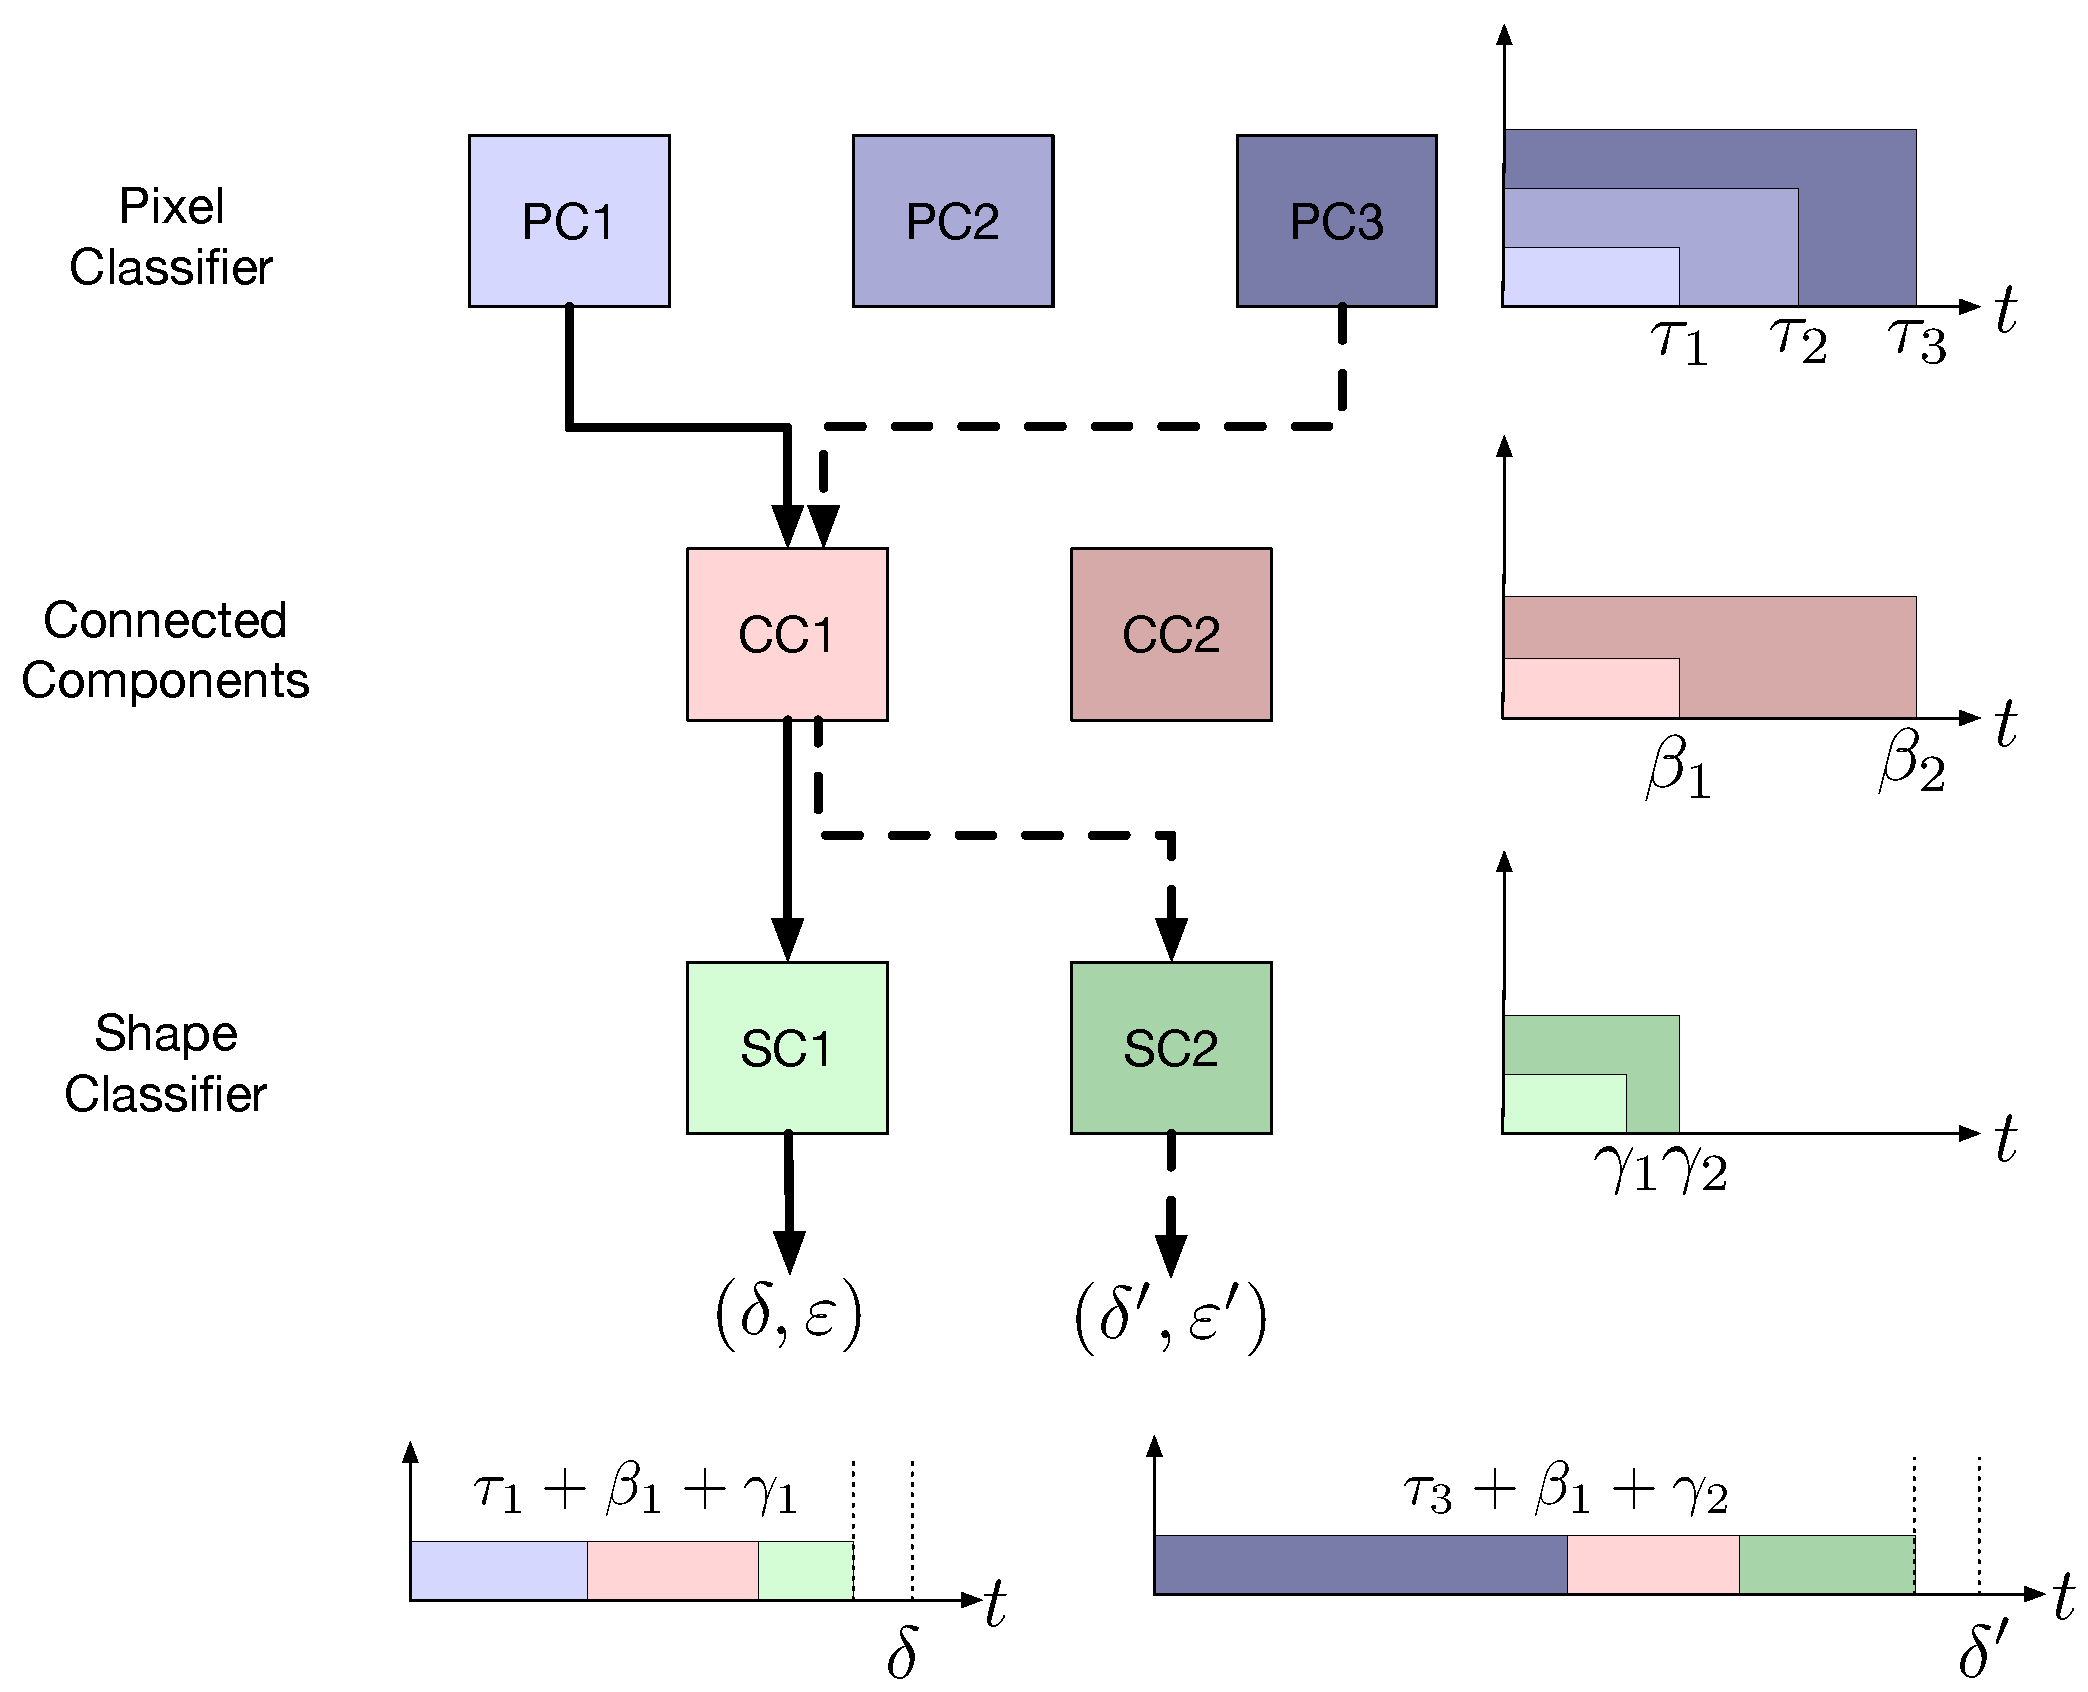
\includegraphics[width=0.49\textwidth]{Figures/real_time_figure.pdf}
	\caption{A perception algorithm for object detection is decomposed into three tasks, and various components used to compose the contract based perception algorithm and their representation as real-time tasks. For a given $\delta$ contract, knob settings are chosen at run-time resulting in a schedule to execute these sequential components, or tasks, to respect the contract. }
	\label{fig:offline}
\end{figure}

\subsection{Contract-based Co-design of Anytime Computation and Robust Control}
Anytime algorithms \cite{boddy} are a class of algorithms that can be interrupted at any point during their execution and still return a usable solution, usually one whose quality is monotonically improving with time. 
\emph{Contract algorithms} \cite{zilbersteinAImag} are a version of anytime algorithms where the interruption time is chosen from a set of pre-defined times. 
%The use of such algorithms for the computationally heavy perception and estimation algorithms would give a level of flexibility with a computation time/quality trade-off that is not offered by run-to-completion algorithms. In general, most perception and estimation algorithms do not lend themselves to such implementations.
In our recent work \cite{RTSS15, Complex15}, we show how to convert off-the-shelf P\&SE algorithms into \emph{contract algorithms}, and how to design a controller that takes advantage of this capability.

%\mynote{HA}{Way too contrived, Yash...say things more plainly, in the active voice. The next paragraph doesn't actually give any information, it's a string of words. Example: what does "realization" mean? testing? design? implementation? analysis? if there's a more precise word, use it. if there isn't, explain what you mean by it.}
\begin{figure}[t]
	\centering
	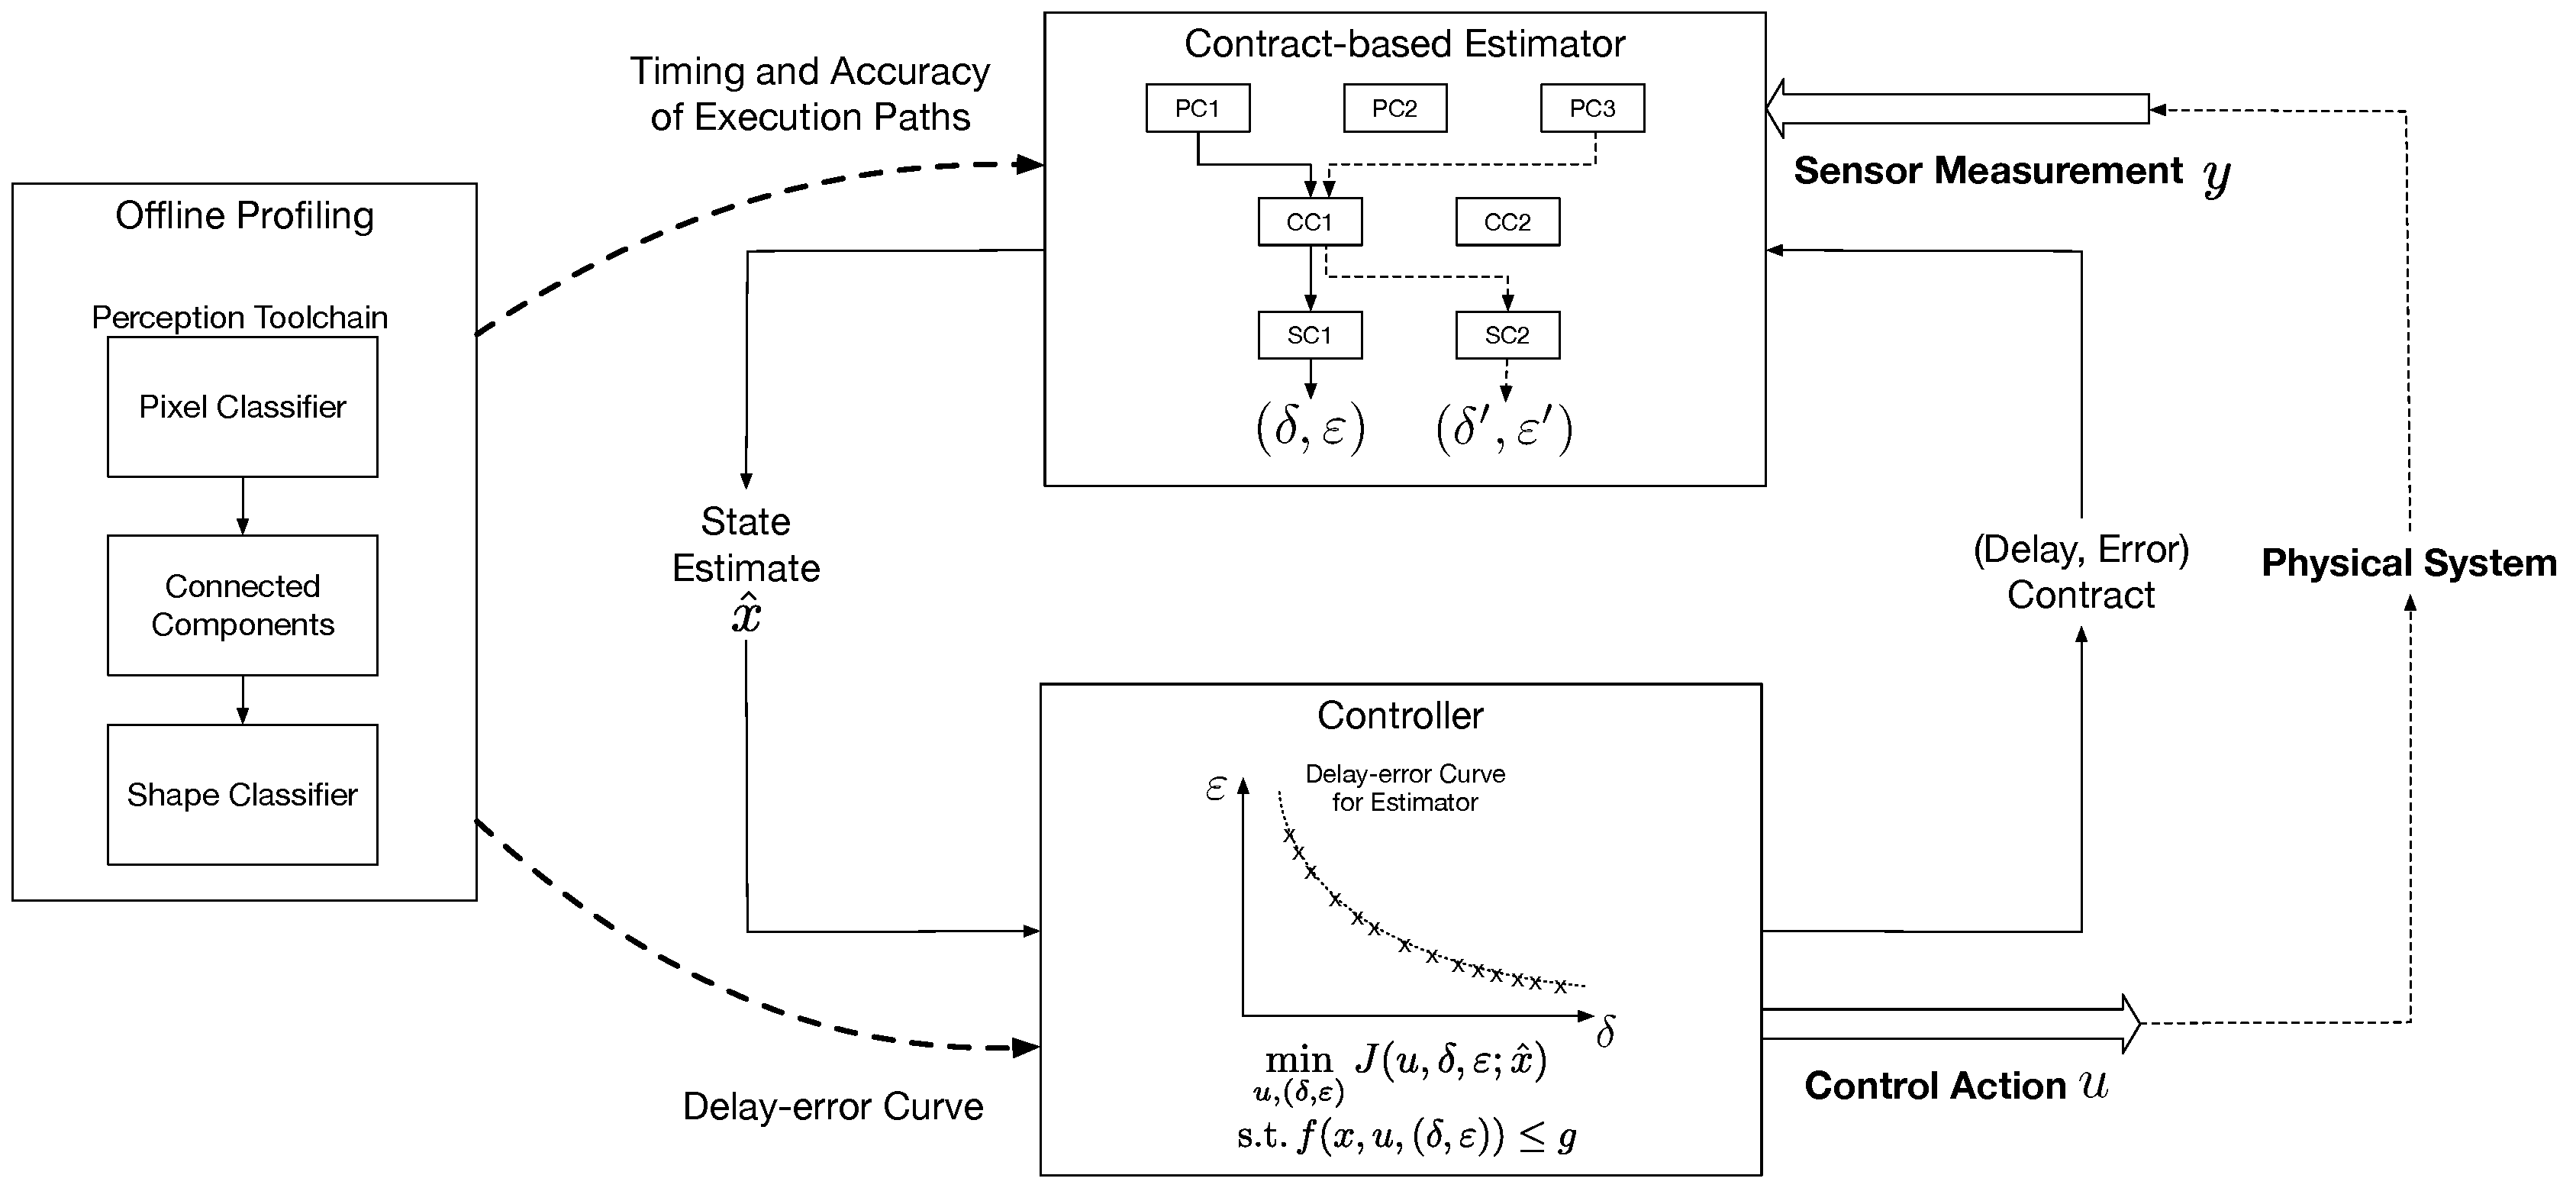
\includegraphics[width=0.49\textwidth]{Figures/process_figure2.pdf}
	\caption{Contract-based estimator and controller. This differs from regular state-estimation based feedback control as the controller can set contracts (deadlines) for the perception/estimation algorithm. Based on the contract and the offline profiling, the contract based estimator decides at run-time what tasks to execute in order to best meet the contract.}
	\label{fig:fullcodesignedCE}
	\vspace{-10pt}
\end{figure}

First, the PS\&E is profiled off-line.
Namely, the algorithm's parameters are varied and for each setting of the parameters, it is run on a \emph{profiling data set}. 
This yields a finite set of \emph{contracts}: a contract is a pair (estimation delay, estimation error), and each setting of the parameters yields one contract when run on the profiling data set
Fig. \ref{fig:offline} shows this approach applied to an object detection algorithm.
At run-time, when the estimator receives a (delay, error) contract request from the controller, it can adapt its execution paths to respect the contract, namely, to provide a state estimate within the requested error bound, and within the requested delay.
Another dimension of decision making, explored in \cite{Complex15}, is resource allocation for execution of tasks, e.g. whether the task gets executed on the CPU or the GPU, resulting in a power versus computation delay trade-off.

The controller is designed with the knowledge of the contracts that can be realized by the P\&SE algorithm, and at each time step will request a contract.
This gives the controller the ability to leverage the flexible nature of the estimation algorithm to maximize some measure of control performance. %\todo[inline]{Might want to avoid mentioning \emph{separability principle}}
In \cite{RTSS15} we develop a Robust Model Predictive Control algorithm that can leverage this trade-off offered by the contract based co-design (see Fig. \ref{fig:fullcodesignedCE} while optimizing for a joint cost of control performance and computation power consumption. We experimentally evaluated our approach on a hex-rotor with visual odometry and showed improved control performance and computation energy efficiency over a baseline MPC controller that does not leverage co-design.


Fig.~\ref{fig:fullcodesignedCE} shows the closed loop architecture in a system with co-design of the anytime computation (estimator) and robust controller.
In the co-designed system as presented in this paper, the controller can make the estimation algorithm switch to lower or higher time (and/or energy) consuming modes based on the control objective at the current time step.
The main components of the co-design architecture are a contract based perception-and-estimation algorithm, a robust control algorithm that computes an input to be sent to the physical system being controller as well as the operating mode for the contract time estimator, and the interface between them. More details on these components are in the following sections.






%\section{Conclusion}
%The conclusion goes here.




% conference papers do not normally have an appendix


% use section* for acknowledgment
%%\section*{Acknowledgment}


%%The authors would like to thank...





% trigger a \newpage just before the given reference
% number - used to balance the columns on the last page
% adjust value as needed - may need to be readjusted if
% the document is modified later
%\IEEEtriggeratref{8}
% The "triggered" command can be changed if desired:
%\IEEEtriggercmd{\enlargethispage{-5in}}

% references section

% can use a bibliography generated by BibTeX as a .bbl file
% BibTeX documentation can be easily obtained at:
% http://mirror.ctan.org/biblio/bibtex/contrib/doc/
% The IEEEtran BibTeX style support page is at:
% http://www.michaelshell.org/tex/ieeetran/bibtex/
%\bibliographystyle{IEEEtran}
% argument is your BibTeX string definitions and bibliography database(s)
%\bibliography{IEEEabrv,../bib/paper}
%
% <OR> manually copy in the resultant .bbl file
% set second argument of \begin to the number of references
% (used to reserve space for the reference number labels box)
%\begin{thebibliography}{1}

%\bibitem{IEEEhowto:kopka}
%H.~Kopka and P.~W. Daly, \emph{A Guide to \LaTeX}, %3rd~ed.\hskip 1em plus
%  0.5em minus 0.4em\relax Harlow, England: Addison-Wesley, 1999.

%\end{thebibliography}

% Add you bibliographic information here...
\bibliographystyle{unsrt}
\bibliography{bibliography,bibliography2,IEEEabrv,mok,AnytimeBib,dataCPESrefs,WCNbibliography}




% that's all folks
\end{document}


